%
% $Id: $
%
%
% Compilar a .pdf con LaTeX (pdflatex)
% Es necesario instalar Beamer (paquete latex-beamer en Debian)
%

%
% Gráficos:
% Los gráficos pueden suministrarse en PNG, JPG, TIF, PDF, MPS
% Los EPS deben convertirse a PDF (usar epstopdf)
%


\documentclass[17pt,aspectratio=169,hyperref=pdfusetitle]{beamer}
\usetheme[orchid]{Hannover}
\beamertemplatenavigationsymbolsempty
\setbeamertemplate{headline}{}
\useoutertheme{infolines}

\usepackage[spanish]{babel}
\usepackage[utf8]{inputenc}
\usepackage{graphics}
%\usepackage{amssymb} % Simbolos matematicos
%\usepackage[pdfusetitle]{hyperref}

%\usepackage{chronosys}

%% two slides per page
%\usepackage{pgfpages}
%\pgfpagesuselayout{2 on 1}[a4paper,border shrink=5mm]

\newcommand\YUGE{\fontsize{48}{60}\selectfont}

%\newcommand{\secimage}{figs/bookpages}
\newcommand{\secimage}{figs/laptop-dashboard}
\AtBeginSection[]
{
  {
    \usebackgroundtemplate{\includegraphics[width=\paperwidth,height=\paperheight]{\secimage}}
    \begin{frame}<beamer>

      \begin{center}
        {\YUGE\bf\insertsection}
      \end{center}
    \end{frame}
  }
}

\begin{document}

\title[Analytics with GrimoireLab]{Software Development Analytics with GrimoireLab}
%\subtitle{}
\author[Jesus M. Gonzalez-Barahona]{Jesus M. Gonzalez-Barahona}
\institute[URJC]{Universidad Rey Juan Carlos \\
  @jgbarah ~~~~~ \url{http://github.com/jgbarah/presentations}}

\date[Visual Software Analytics]{Intl. Summer School on Visual Soft. Analytics \\ Leipzig (Germany), September 23rd 2019}

%\begin{frame}[label=firstframe]
\begin{frame}
  \maketitle
\end{frame}

\begin{frame}

  {\em
    \begin{center}
      It is difficult to improve \\
      if you cannot measure \\
      and track your improvement \\
    \end{center}
  }
\end{frame}


\begin{frame}
\frametitle{Our plan today}

\tableofcontents
\end{frame}

%%---------------------------------------------------------------
%%---------------------------------------------------------------
\section{A bit of context}

%%---------------------------------------------------------------

\begin{frame}
\frametitle{Me and my two hats}

\begin{columns}[T]
\begin{column}{.80\textwidth}

Uni Rey Juan Carlos:

\begin{itemize}
\item Understanding free, open source software
\item Data analytics approach
\item Data visualization in XR
\end{itemize}

\begin{flushright}
\url{http://gsyc.es/jgb}
\end{flushright}

\end{column}%
\hfill%
\begin{column}{.18\textwidth}
  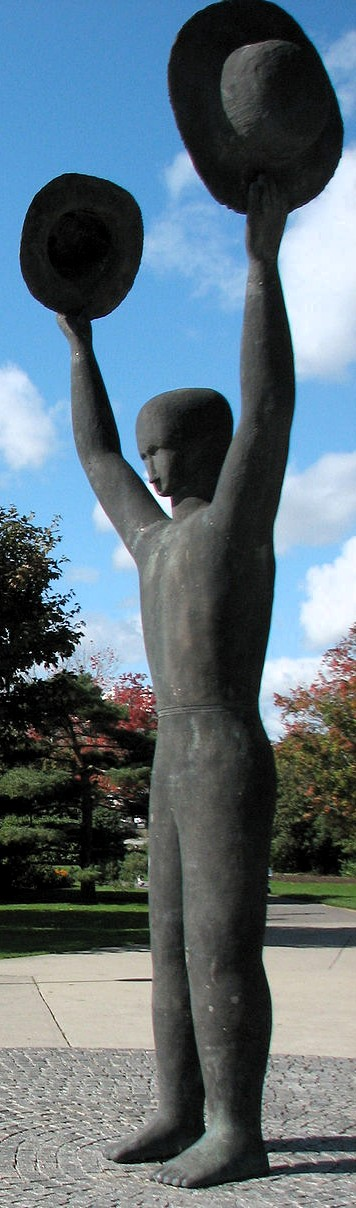
\includegraphics[height=7cm]{figs/two-hats}
\end{column}%
\end{columns}

\end{frame}

%%---------------------------------------------------------------

\begin{frame}
\frametitle{Me and my two hats}

\begin{columns}[T]
\begin{column}{.80\textwidth}

Bitergia:

\begin{itemize}
\item From research to the real world
\item Understanding software development
\item Data analytics approach
\end{itemize}

\begin{flushright}
\url{http://bitergia.com}
\end{flushright}

\end{column}%
\hfill%
\begin{column}{.18\textwidth}
  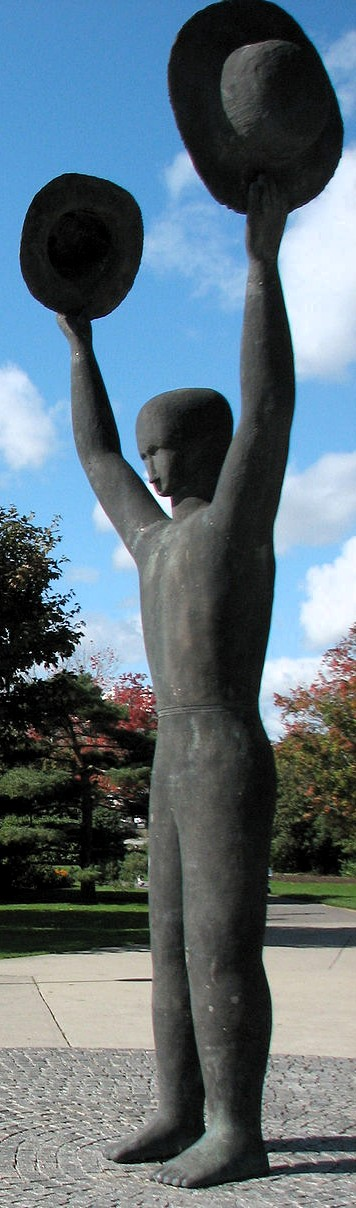
\includegraphics[height=7cm]{figs/two-hats}
\end{column}%
\end{columns}

\end{frame}


%%---------------------------------------------------------------

\begin{frame}
\frametitle{Recommendations}

  \begin{itemize}
  \item Open your laptop
  \item Download the slides (they have links)
  \item Visit Alpha.Cauldron.io and produce your own dashboard
  \item Play with the dashboards
  \item Understand the interpretations behind the numbers
  \end{itemize}

  \begin{flushright}
    \url{https:/alpha.cauldron.io}
  \end{flushright}
\end{frame}

%%---------------------------------------------------------------

\begin{frame}
\frametitle{Cauldron Alpha}

\begin{center}
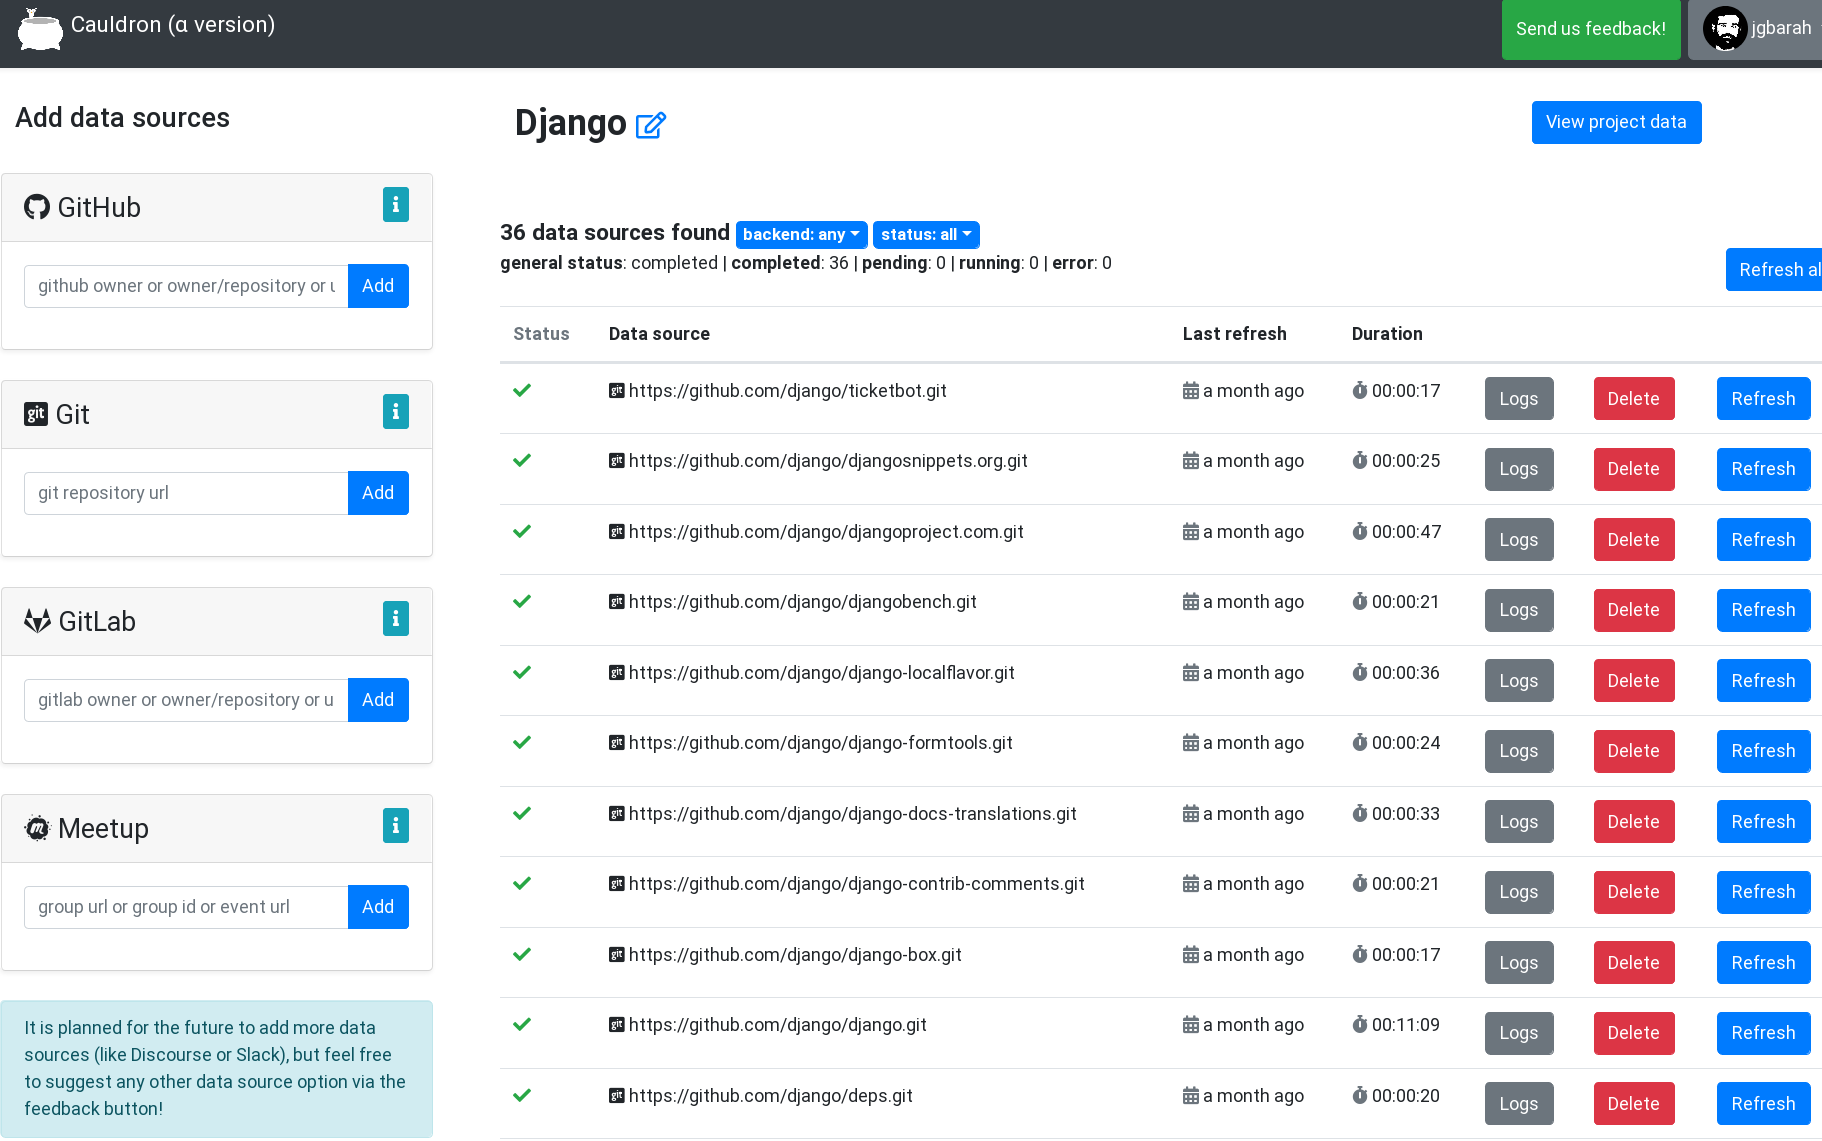
\includegraphics[height=6cm]{figs/cauldron-dashboard}
\end{center}

\end{frame}

%%---------------------------------------------------------------

\begin{frame}
\frametitle{Cauldron Alpha}

\begin{center}
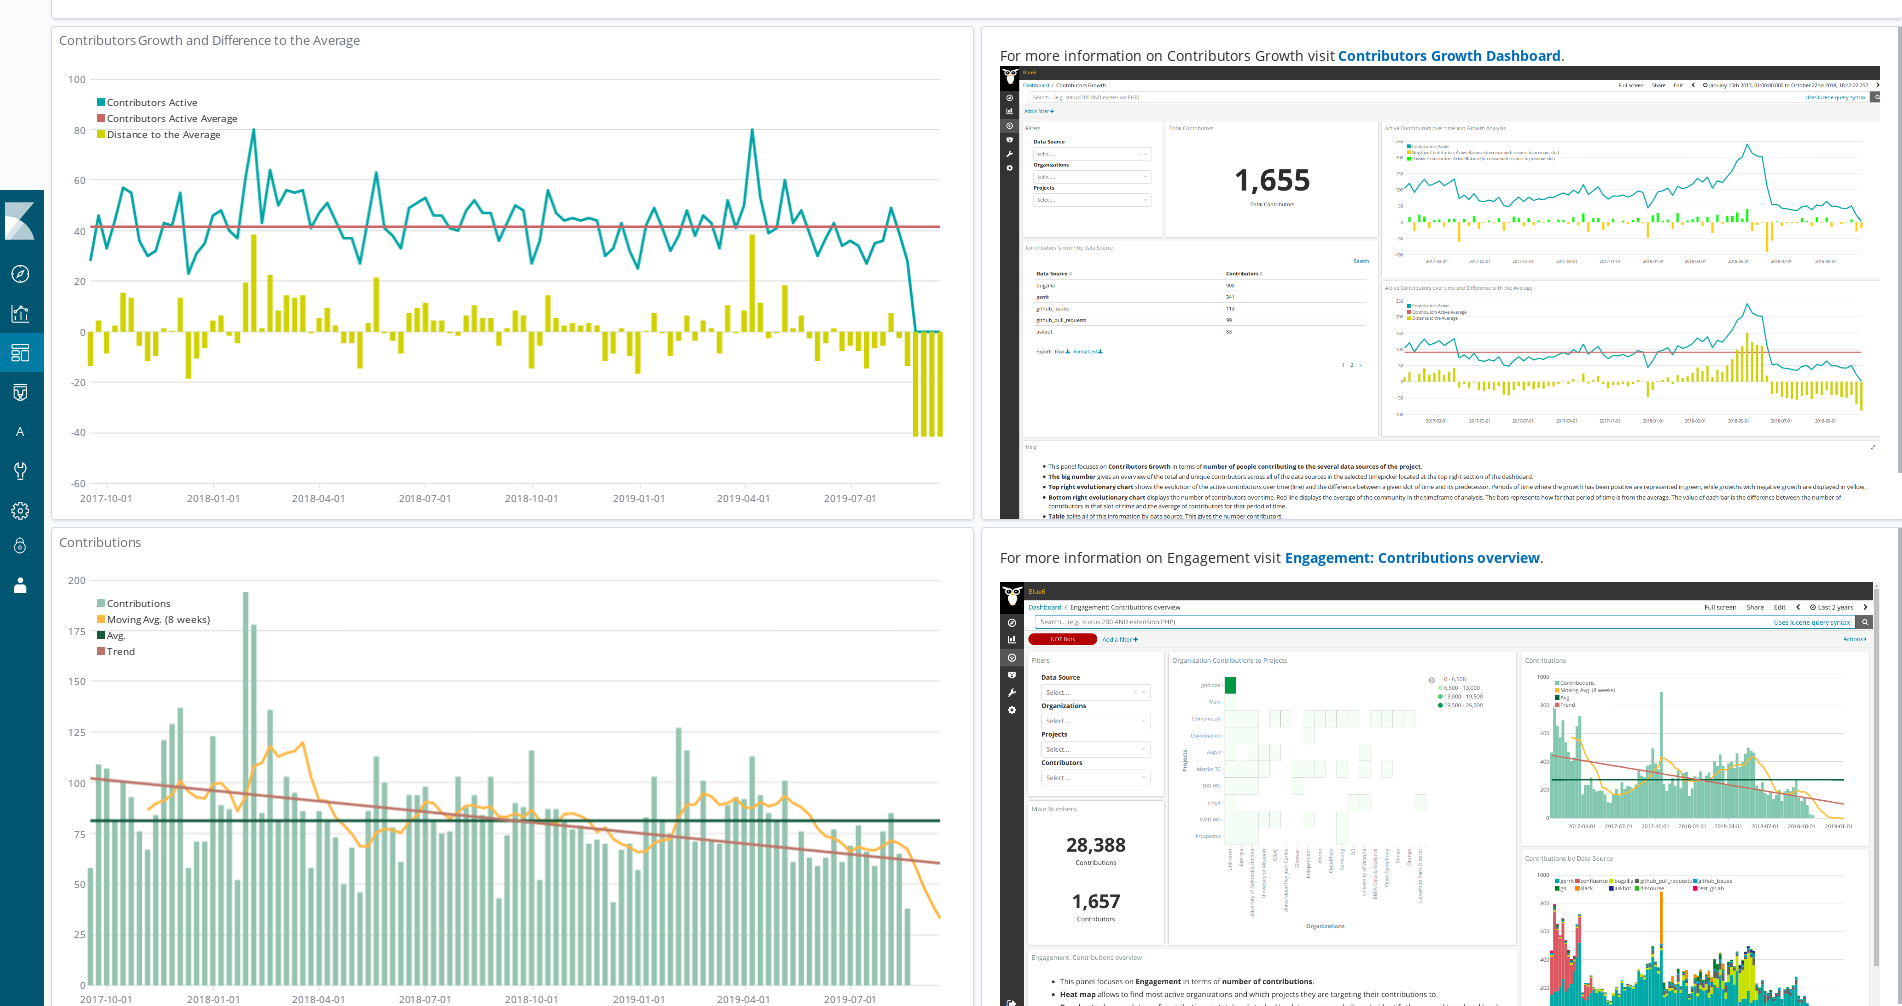
\includegraphics[height=6cm]{figs/cauldron-dashboard-2}
\end{center}

\end{frame}

%%-------------------------------------------------------
%%-------------------------------------------------------
\section{Dealing with dynamic complexity}

%%---------------------------------------------------------------

\begin{frame}
Development projects may be large and complex

\begin{center}
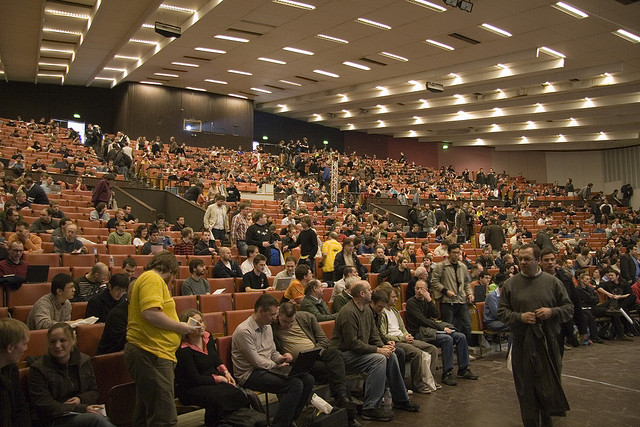
\includegraphics[height=7cm]{figs/fosdem-crowd}
\end{center}

\end{frame}

%%---------------------------------------------------------------

\begin{frame}
\begin{flushright}
  Projects may be large and complex... \\
  and dynamic \\
\end{flushright}

It's difficult to... \

\begin{itemize}
\item ...track what's happening
\item ...understand why it's happening
\item ...react quickly
\item ...evaluate results of reaction 
\end{itemize}

\vspace{.2cm}

\begin{flushright}
If data is available\\
analytics may come to the rescue\\
\end{flushright}

\end{frame}

%%---------------------------------------------------------------

\begin{frame}
\frametitle{A continuous process}

Figure out your interest \\
Find out available data \\
Define key parameters \\
Monitor, understand, detect deviations \\
Act to correct, improve \\
Track results \\

\begin{flushright}
{\em Measure $\rightarrow$ Monitor $\rightarrow$ Act}
\end{flushright}
\end{frame}

%%---------------------------------------------------------------

\begin{frame}
\frametitle{A continuous process}

\begin{flushright}
Case example: Overall development activity
\end{flushright}

\emph{Interest:} activity \\
\emph{Data:} changes to code, tickets \\
\emph{Parameters:} commits, tickets closed \\
\emph{Monitoring:} charts, numbers
\begin{flushright}
\emph{Observation:} numbers declining \\
\emph{Action:} allocate more developer effort \\
\end{flushright}
\emph{Track results...} \\
\begin{flushright}
Measure $\rightarrow$ Monitor $\rightarrow$ Act
\end{flushright}
\end{frame}


%%-------------------------------------------------------
%%-------------------------------------------------------
\section{Data sources}

%%---------------------------------------------------------------

\begin{frame}
  \frametitle{Repositories, repositories...}

  \begin{center}
    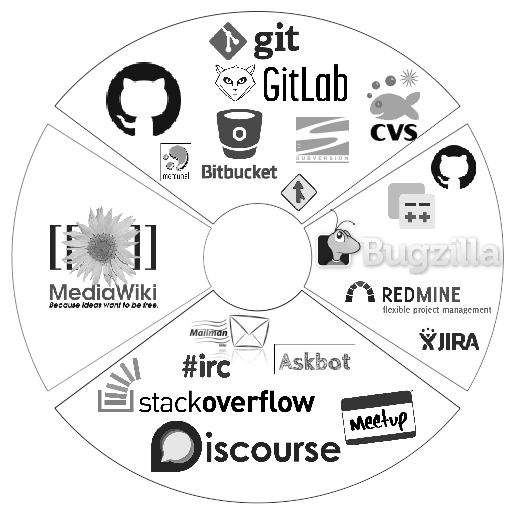
\includegraphics[height=8cm]{figs/data-sources}
  \end{center}
\end{frame}

%%---------------------------------------------------------------

\begin{frame}
\frametitle{Source code management}

\begin{itemize}
\item Client/server: CVS, Subversion
\item Decentralized: git, Mercurial, Bazaar, etc.
\item Most of them accessible through git... \\
  (with some problems)
\item Can be integrated with other tools: \\
  Gerrit, GitHub, GitLab, etc.
\end{itemize}
\end{frame}

%%---------------------------------------------------------------

\begin{frame}
\frametitle{Issue tracking}

Many different systems:

\begin{itemize}
\item Bugzilla
\item Jira
\item GitHub issues
\item GitLab Issues
\item Phabricator
\item RedMine...
\end{itemize}

Each with a different model, data, operations...

\end{frame}


%%---------------------------------------------------------------

\begin{frame}
\frametitle{Code review}

Usually: peer review pre-merge review \\

Different methods: 

  \begin{itemize}
  \item Mailing lists (eg: Linux)
  \item Gerrit (eg: OpenStack)
  \item GitHub pull requests (eg: ElasticSearch)
  \item GitLab merge requests (eg: GNOME)
  \item or even Jira, Bugzilla...
  \end{itemize}

  \begin{flushright}
    Much of the control on the software lies here \\
  \end{flushright}
\end{frame}

%%---------------------------------------------------------------

\begin{frame}
\frametitle{Async communication}

  Mailing lists: \\
  \begin{itemize}
  \item Mailing lists systems (Mailman)
  \item Google Groups
  \item Mailing list archivers
  \end{itemize}

  Forums: too many to mention \\

  Question/Answer sites: StackOverflow, Askbot  \\

  \begin{flushright}
    Information is always archived
  \end{flushright}
\end{frame}

%%---------------------------------------------------------------

\begin{frame}
\frametitle{Sync communication}

  Systems:

  \begin{itemize}
  \item Traditionally: IRC
  \item Nowadays: Slack \& many others
  \item Not always text/based (eg: videoconferences)
  \end{itemize}
  
  Notes:
  
  \begin{itemize}
  \item In many cases, lack of archives
  \item Privacy concerns: considered informal communication
  \item Difficult to track identities
  \end{itemize}
\end{frame}

%%---------------------------------------------------------------
%%---------------------------------------------------------------
\section{GrimoireLab}

%%---------------------------------------------------------------
%% \begin{frame}

%% \begin{center}
%%   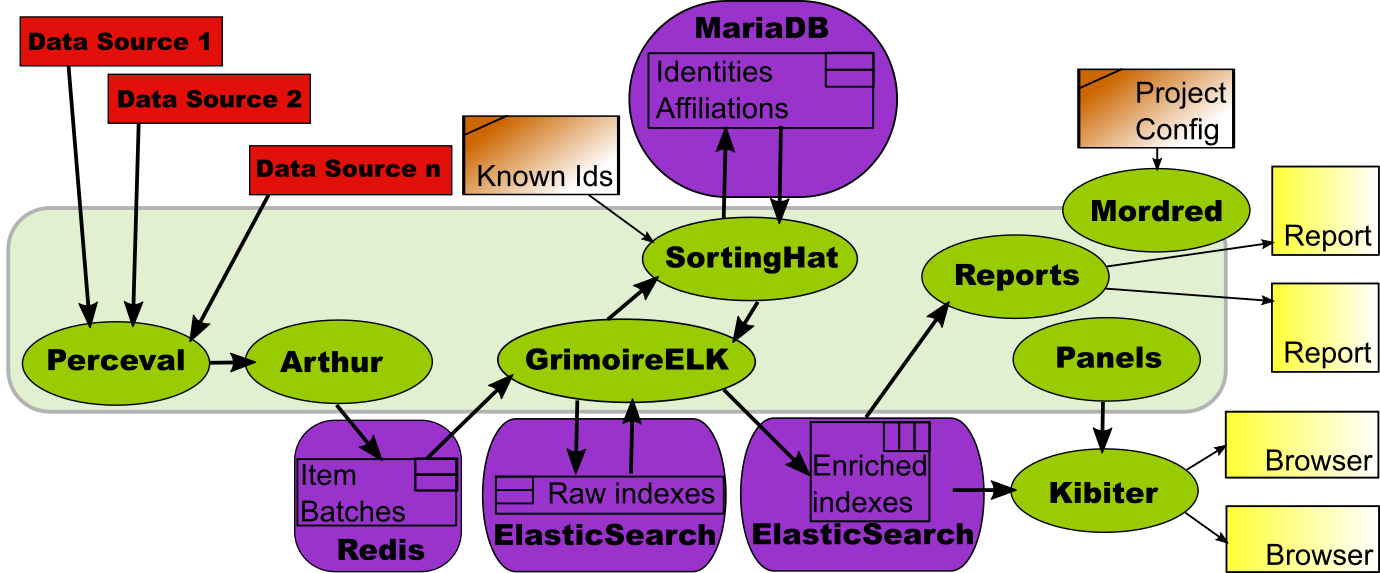
\includegraphics[width=12cm]{figs/grimoirelab-all-complete}
%% \end{center}

%% \begin{flushright}
%%   \url{https://chaoss.github.io/grimoirelab}
%% \end{flushright}
%% \end{frame}

%%---------------------------------------------------------------

\begin{frame}


  
\includegraphics[width=12cm]{figs/grimoirelab}

  \begin{flushright}
  \url{https://chaoss.github.io/grimoirelab}
  \end{flushright}

\end{frame}


%%---------------------------------------------------------------
\begin{frame}

\begin{center}
  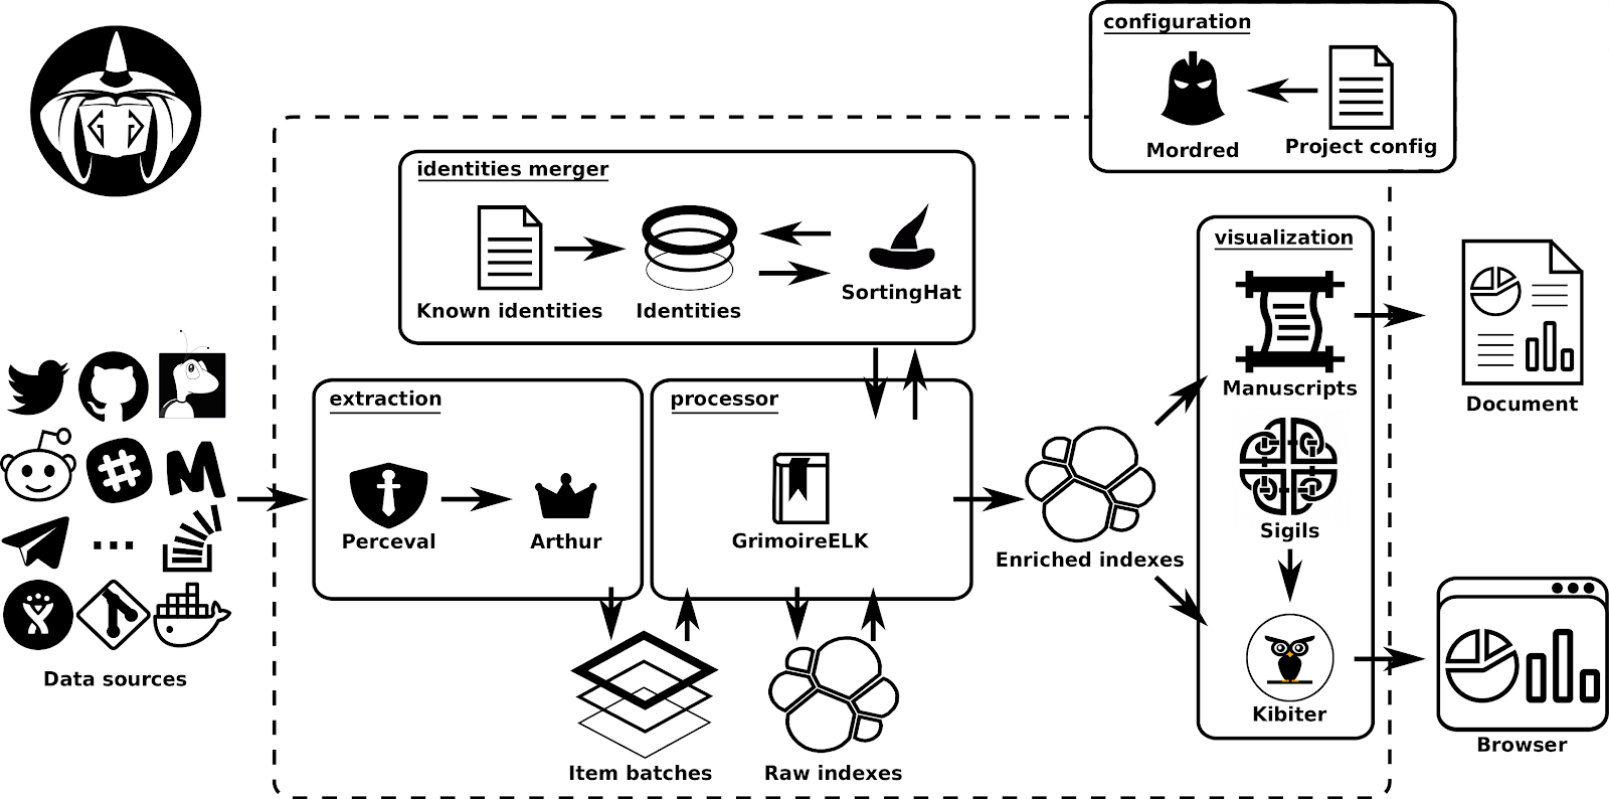
\includegraphics[width=12cm]{figs/grimoirelab-arquitecture}
\end{center}

\begin{flushright}
  \url{https://chaoss.github.io/grimoirelab}
\end{flushright}
\end{frame}

%%---------------------------------------------------------------

\begin{frame}
\frametitle{Main components}

  \begin{itemize}
  \item Perceval: data retrieval
  \item Arthur: retrieval orchestration
  \item GelK: enrichment
  \item SortingHat: identity management
  \item ElasticSearch (*): database
  \item Kibiter: dashboard (light fork of Kibana)
  \item Sigils: visualizations for Kibana/Kibiter
  \end{itemize}

  (*) Not a part of GrimoireLab

\end{frame}

%%---------------------------------------------------------------

\begin{frame}[fragile]
\frametitle{Perceval}

{\small
\begin{verbatim}
$ python3 -m venv gl
$ source gl/bin/activate
(gl) $ pip install grimoirelab
(gl) $ perceval git \
  https://github.com/chaoss/grimoirelab-perceval
(gl) $ perceval github \
  chaoss grimoirelab-perceval
\end{verbatim}
}

\vspace{1cm}
{\footnotesize
\begin{flushright}
  \href{chaoss.github.io/grimoirelab-tutorial/perceval}{https://chaoss.github.io/grimoirelab-tutorial/perceval}
\end{flushright}
}
\end{frame}

%%---------------------------------------------------------------

\begin{frame}[fragile]

{\footnotesize
\begin{verbatim}
{"backend_name": "Git",
"backend_version": "0.11.1",
"category": "commit",
"classified_fields_filtered": null,
"data": {
  "Author": "Santiago Due\u00f1as <sduenas@bitergia.com>",
  "AuthorDate": "Tue Aug 18 18:08:27 2015 +0200",
  "Commit": "Santiago Due\u00f1as <sduenas@bitergia.com>",
  "CommitDate": "Tue Aug 18 18:08:27 2015 +0200",
  "commit": "dc78c254e464ff334892e0448a23e4cfbfc637a3",
  "files": [{
     "action": "A",
     "added": "10",
     "file": ".gitignore",
\end{verbatim}
}
\end{frame}

%%---------------------------------------------------------------

\begin{frame}[fragile]

{\footnotesize
\begin{verbatim}
{"backend_name": "GitHub",
"backend_version": "0.22.1",
"category": "issue",
"classified_fields_filtered": null,
"assignee_data": {},
"assignees": [],
"assignees_data": [],
"author_association": "CONTRIBUTOR",
"body": "Based on Sphynx, prepared...",
"closed_at": "2016-01-04T13:51:56Z",
"comments": 0,
"comments_data": [],
"comments_url": "https://api.github.com/...",
"created_at": "2016-01-03T23:46:04Z",
\end{verbatim}
}
\end{frame}

%%---------------------------------------------------------------

\begin{frame}[fragile]
  \frametitle{Perceval as a module}
  
{\footnotesize
\begin{verbatim}
#! /usr/bin/env python3
from perceval.backends.core.git import Git

repo_url = 'http://github.com/chaos/grimoirelab-perceval'
repo_dir = '/tmp/perceval.git'

repo = Git(uri=repo_url, gitpath=repo_dir)
for commit in repo.fetch():
    print(commit['data']['commit'])
\end{verbatim}
}
\end{frame}

%%---------------------------------------------------------------

\begin{frame}[fragile]
  
{\footnotesize
\begin{verbatim}
import argparse
from perceval.backends.core.git import Git

parser = argparse.ArgumentParser(description = "Count commits in a git repo")
parser.add_argument("repo", help = "Repository url")
parser.add_argument("--print", action='store_true', help = "Print hashes")
args = parser.parse_args()

repo = Git(uri=args.repo, gitpath='/tmp/perceval.git')
count = 0
for commit in repo.fetch():
    if args.print:
        print(commit['data']['commit'])
    count += 1
print("Number of commmits: %d." % count)
\end{verbatim}
}
\end{frame}

%%---------------------------------------------------------------

\begin{frame}[fragile]
\frametitle{SirMordred}

Producing a dashboard:

\begin{itemize}
\item Elasticsearch installed
\item Kibana / Kibiter installed
\item MariaDB installed
\item Config: mordred.cfg, projects.json, \\
  identities.yaml, menu.yaml
\end{itemize}

{\small
\begin{verbatim}
(gl) $ mordred -c mordred.cfg
\end{verbatim}
}

{\footnotesize
\begin{flushright}
  \href{chaoss.github.io/grimoirelab-tutorial/sirmordred}{https://chaoss.github.io/grimoirelab-tutorial/sirmordred}
\end{flushright}
}
\end{frame}

%%---------------------------------------------------------------

\begin{frame}


  
\includegraphics[width=12cm]{figs/grimoirelab-slide}

\end{frame}

%%---------------------------------------------------------------
%%---------------------------------------------------------------
\section{Case studies}

%%---------------------------------------------------------------

\begin{frame}
\frametitle{Tracking involved parties}

  Development is much more than developers \\
  (this is explicit in FOSS \& inner sourcing)
  
  \begin{itemize}
  \item Developers: all repositories
  \item Contributors: issue tracking, async communication
  \item Users: async communication, ...
  \item Ecosystem: difficult to track
  \end{itemize}

  \vspace{1cm}
  
  Software may include beacons: tracking usage \\

  Needed: tracking identities in different data sources \\
\end{frame}

%%---------------------------------------------------------------
%%---------------------------------------------------------------
\subsection{Activity}

%%---------------------------------------------------------------

\begin{frame}
\frametitle{Activity / size}

  \begin{itemize}
  \item committing patches: \\
    source code management system
  \item reporting, commenting or fixing bugs: \\
    issue tracking system
  \item submitting patches or reviewing them: \\
    code review system
  \item sending messages: \\
    async or sync communication systems
  \end{itemize}
\end{frame}

%%---------------------------------------------------------------

\begin{frame}
\frametitle{Most common cases}

  \begin{itemize}
  \item Parameters reflecting activity for a period.
  \item People active for a certain period.
  \item Evolution of any of them.
  \item Trends for any of them.
  \end{itemize}
\vspace{.5cm}

\begin{flushright}
  Difficult to compare between projects \\  
  Interesting to compare in-project \\
\end{flushright}
\end{frame}

%%---------------------------------------------------------------

\begin{frame}
\frametitle{Many facets}

\begin{center}
  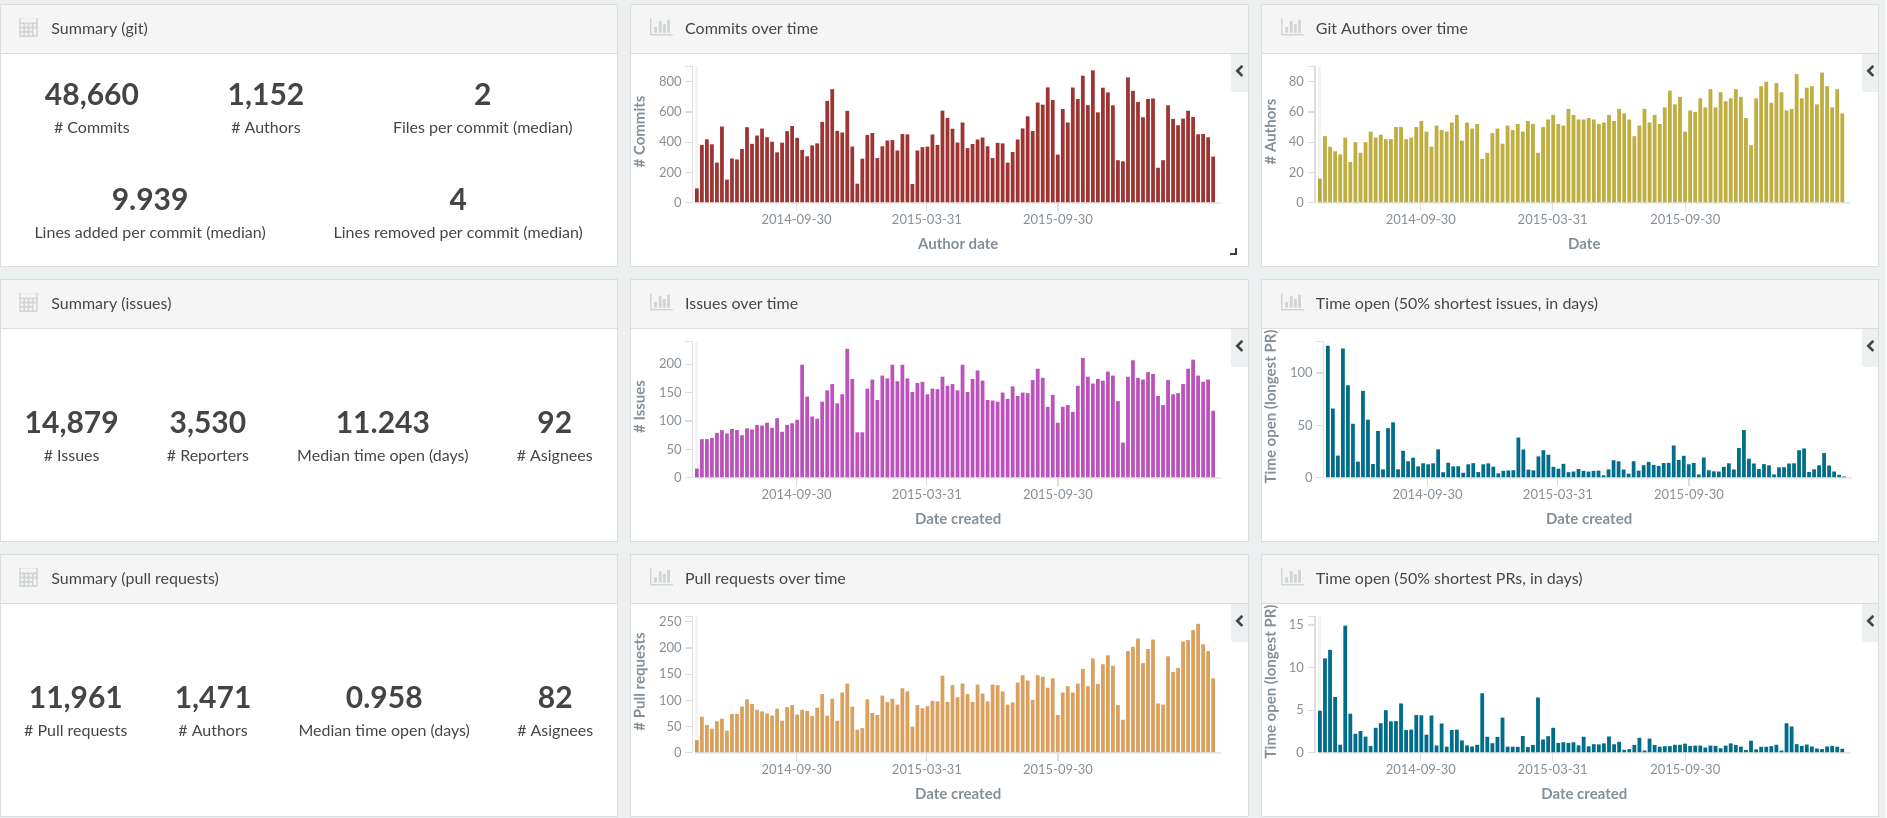
\includegraphics[width=12cm]{figs/activity-elastic}
  
\end{center}

\end{frame}

%%---------------------------------------------------------------

\begin{frame}
\frametitle{Many facets}

\begin{center}
  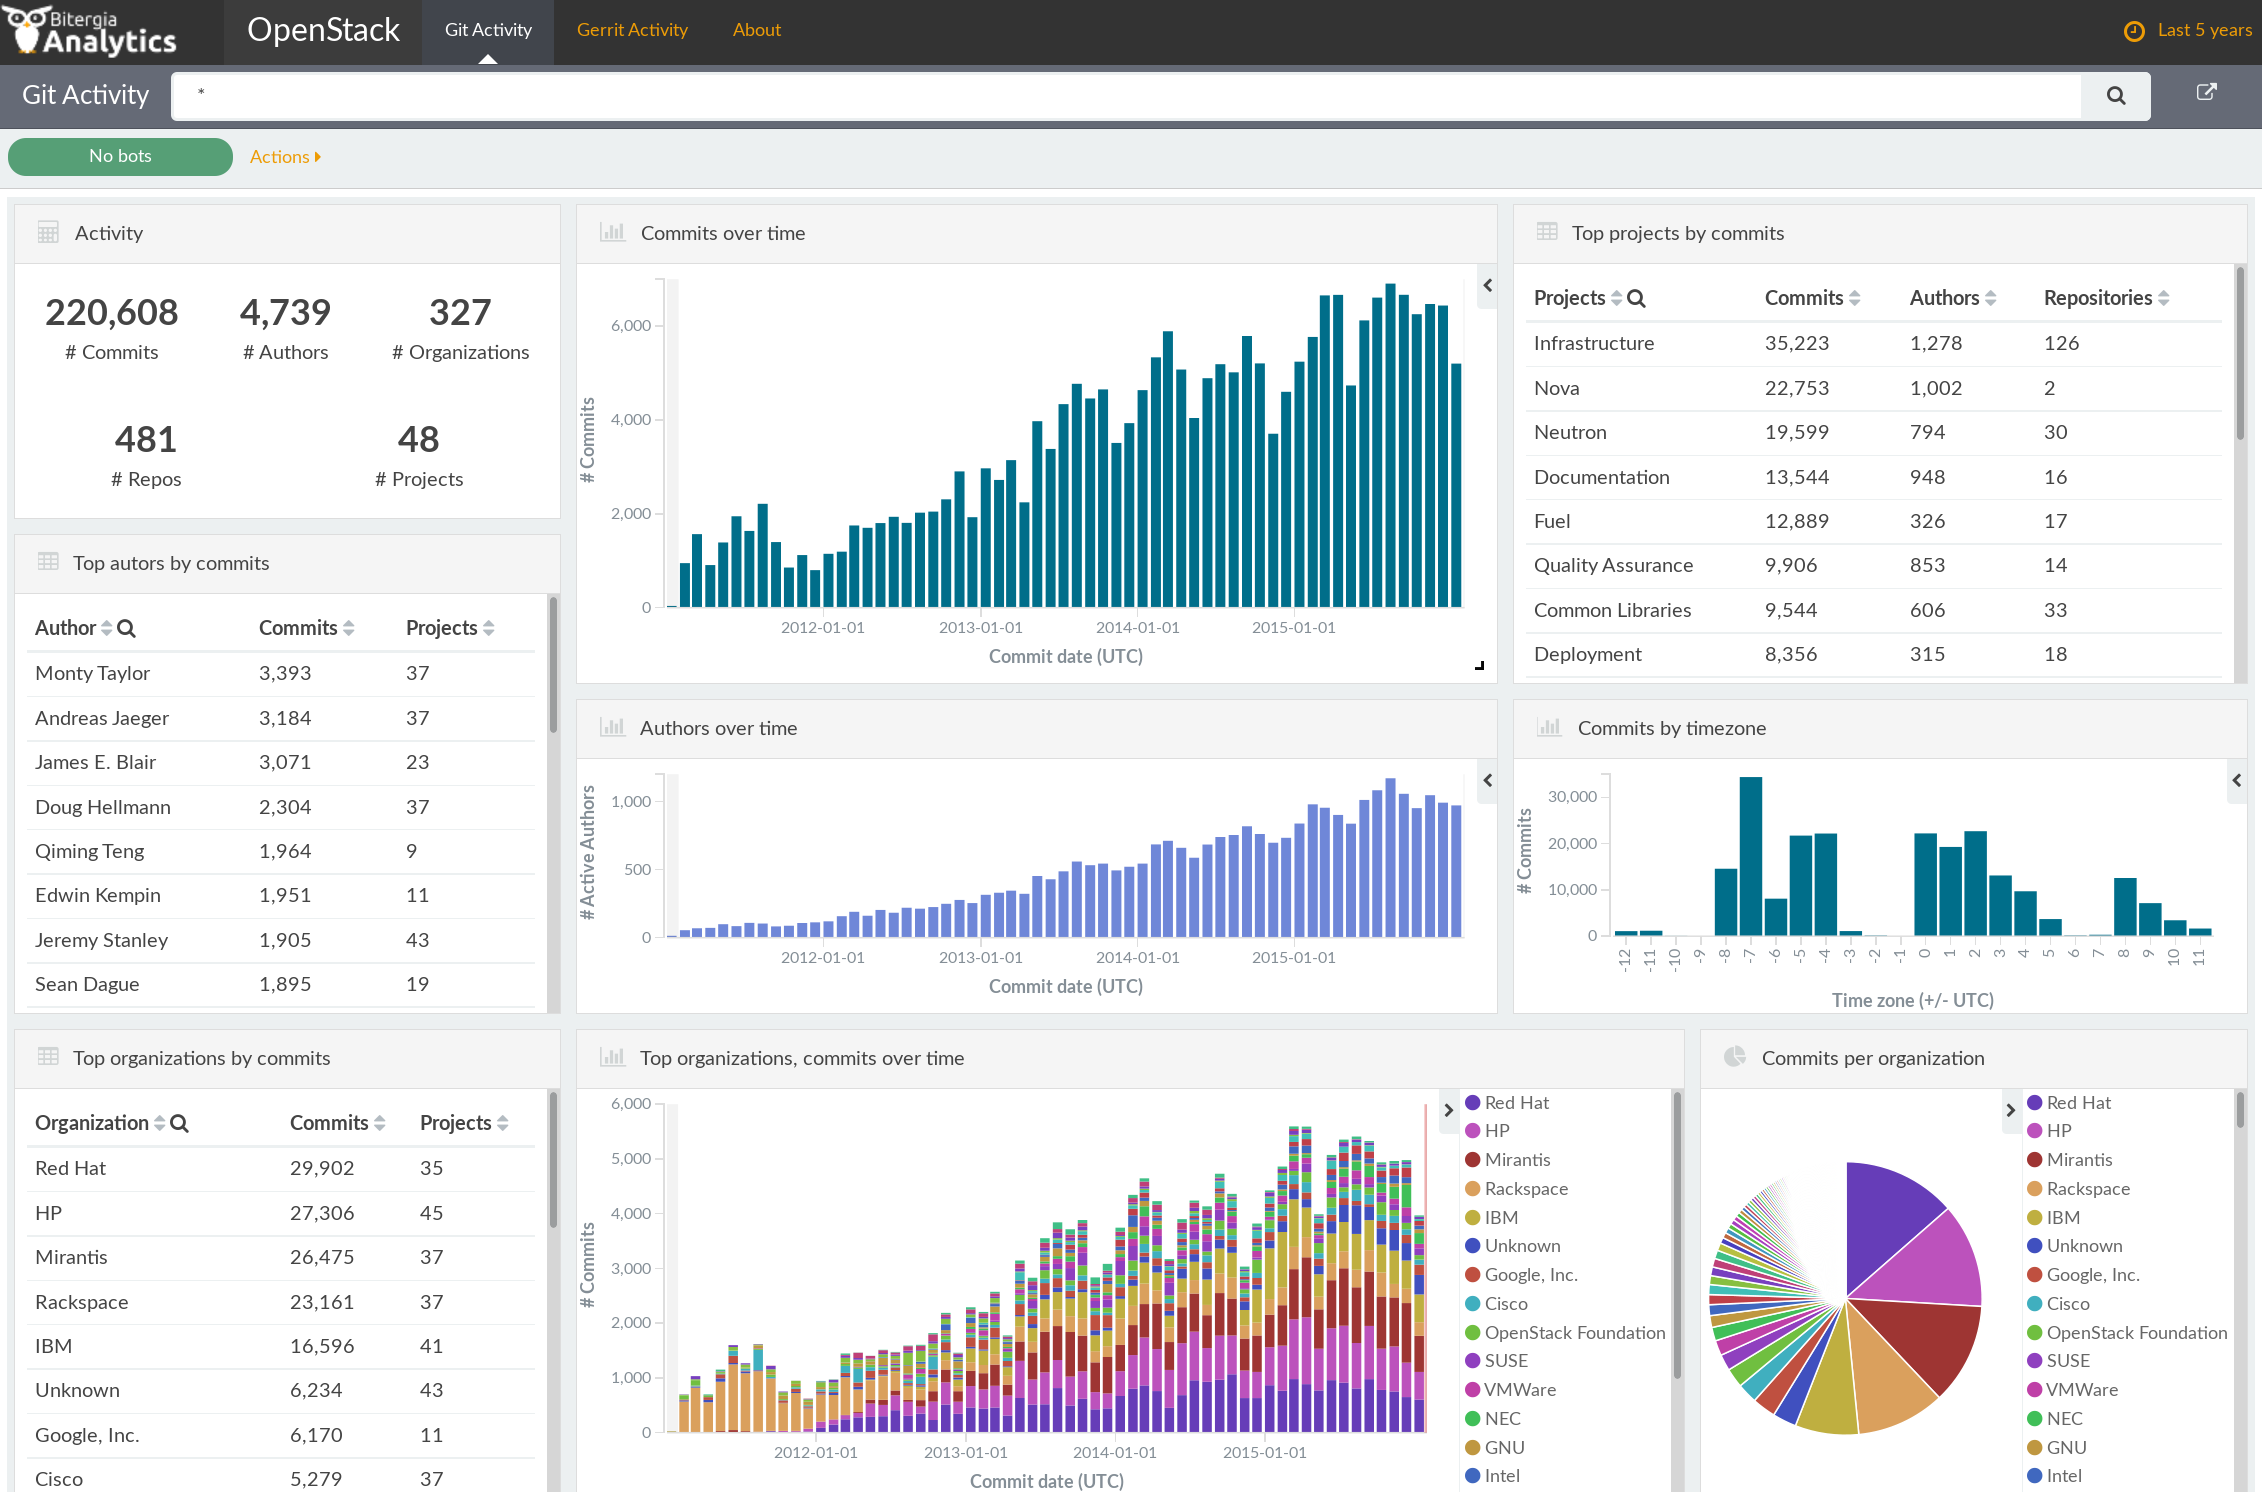
\includegraphics[height=7cm]{figs/bitergia-analytics-fosdem16}
\end{center}

\end{frame}

%%-------------------------------------------------------
%%-------------------------------------------------------
\subsection{Remaining code}

%%---------------------------------------------------------------
\begin{frame}
  \frametitle{How old is code?}
  
\begin{center}
  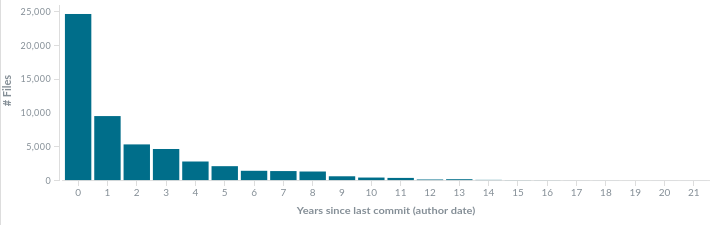
\includegraphics[width=12cm]{figs/linux-files-age}
\end{center}

[Linux kernel, July 2016, C files by last commit]

\end{frame}

%%---------------------------------------------------------------
\begin{frame}

\begin{center}
  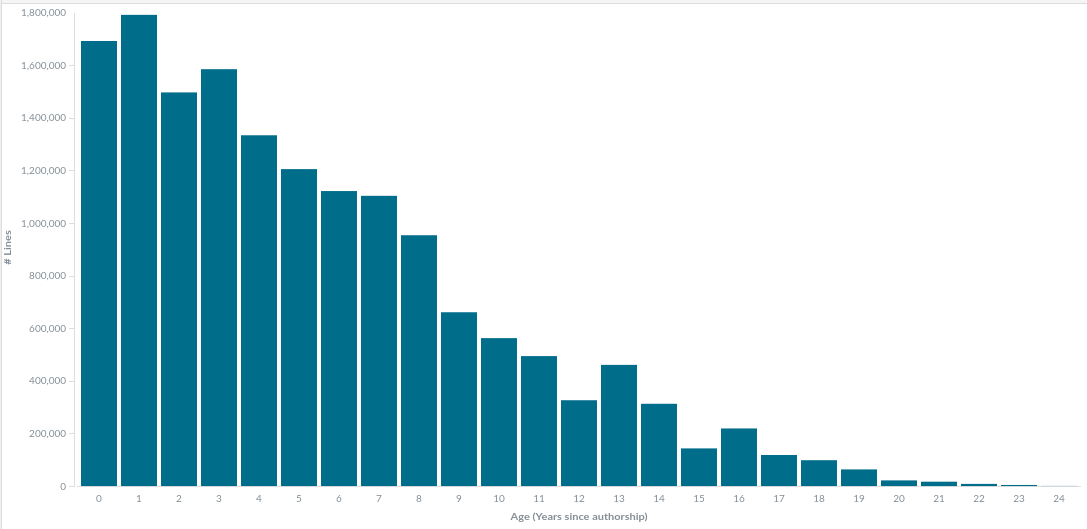
\includegraphics[width=12cm]{figs/linux-age-c}
\end{center}

[Linux kernel, July 2016, lines in C files by age]

\end{frame}

%%---------------------------------------------------------------
\begin{frame}
\frametitle{How old is code (3)}

\begin{center}
  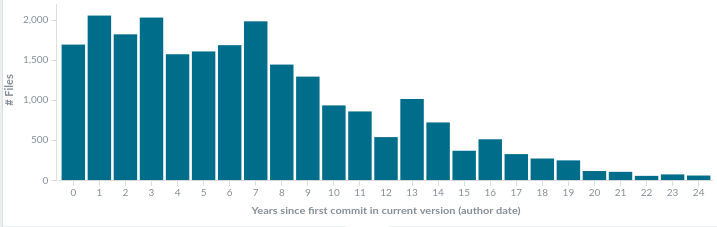
\includegraphics[width=12cm]{figs/linux-files-first-edit-c}
\end{center}

[Linux kernel, July 2016, C files by first remaining commit]

\end{frame}

%%---------------------------------------------------------------
\begin{frame}

\begin{columns}[T]
\begin{column}{.48\textwidth}

  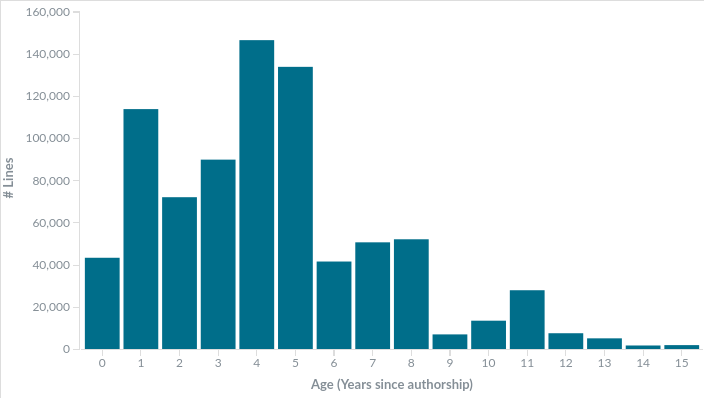
\includegraphics[height=3.1cm]{figs/linux-age-net-wireless-c}

  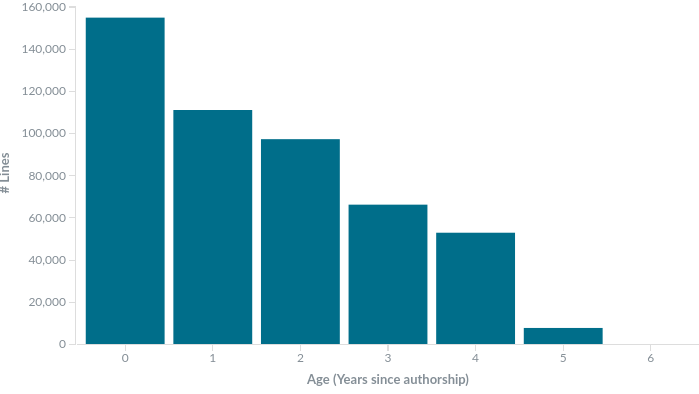
\includegraphics[height=3.1cm]{figs/linux-age-net-ethernet-c}

\end{column}%
\hfill%
\begin{column}{.50\textwidth}

  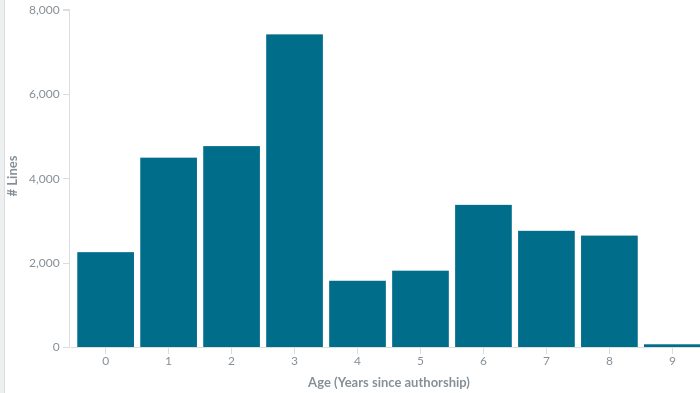
\includegraphics[height=3.1cm]{figs/linux-age-net-usb-c}

  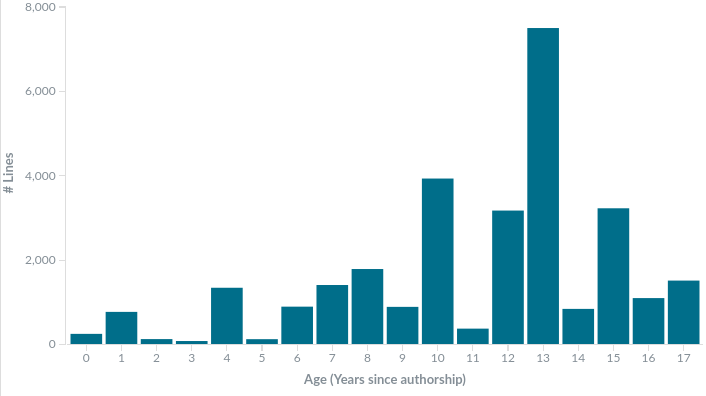
\includegraphics[height=3.1cm]{figs/linux-age-net-irda-c}

\end{column}%
\end{columns}
  
{\small
  Age of lines (data of authorship, ``.c'' files in Linux) \\
From top left, clockwise: Wireless, USB, IRDA Ethernet
}
\end{frame}

%%-------------------------------------------------------
%%-------------------------------------------------------
\subsection{Performance}

%%---------------------------------------------------------------

\begin{frame}
\frametitle{Performance (backlog)}

\begin{center}
  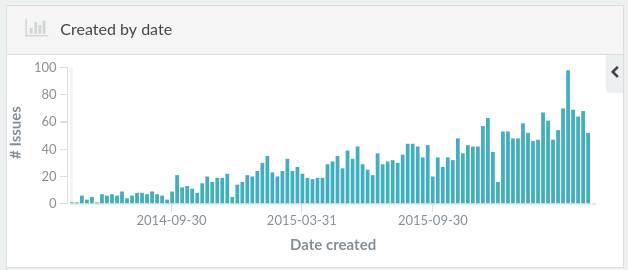
\includegraphics[width=12cm]{figs/backlog-issues-elastic}
\end{center}

Example: backlog of open issues.

\begin{flushright}
  \url{http://cauldron.io/dashboards/elastic}
\end{flushright}

\end{frame}


%%---------------------------------------------------------------

\begin{frame}

\begin{center}
  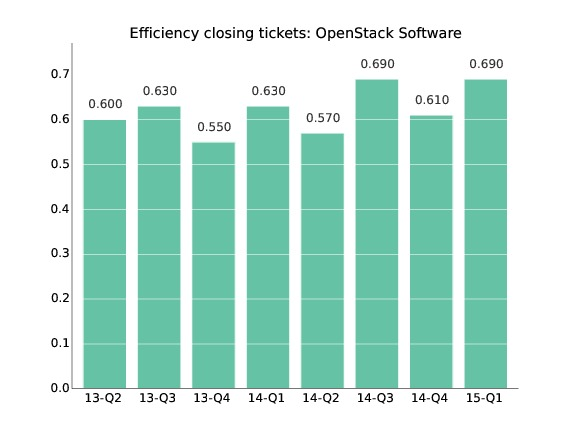
\includegraphics[height=6.5cm]{figs/bmiOpenStackSoftware}
\end{center}

{\small
Efficiency.
Example: closed/opened tickets per quarter \\
}
\end{frame}


%%---------------------------------------------------------------

\begin{frame}
\frametitle{Tickets}

\begin{center}
  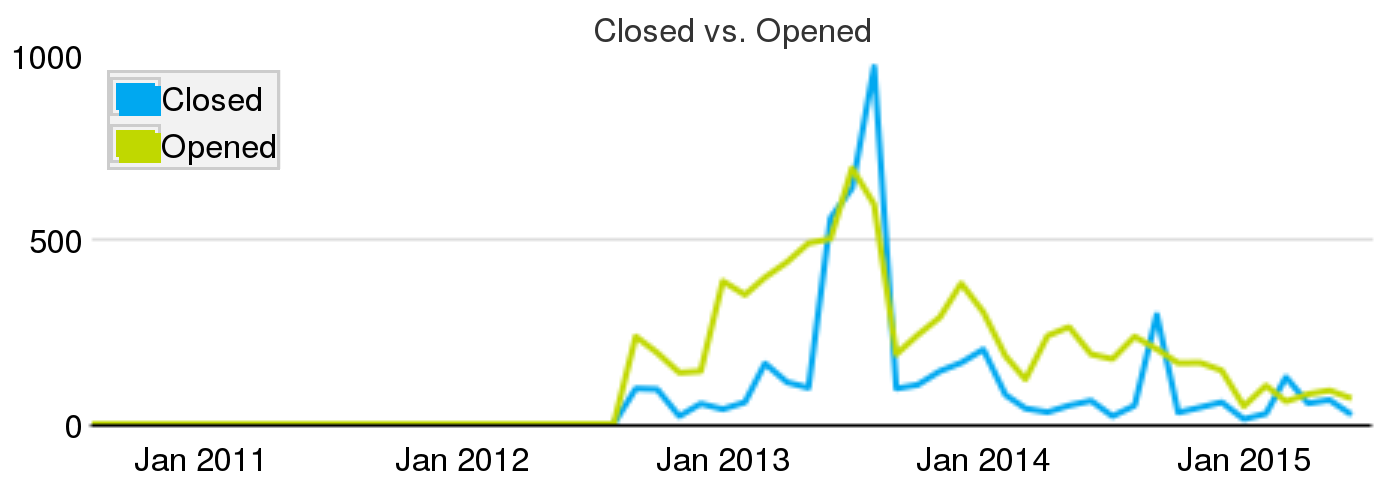
\includegraphics[width=12cm]{figs/processes-tickets-closed-open}
\end{center}

\end{frame}

%%---------------------------------------------------------------

\begin{frame}
\frametitle{Review: time to merge}

\begin{center}
  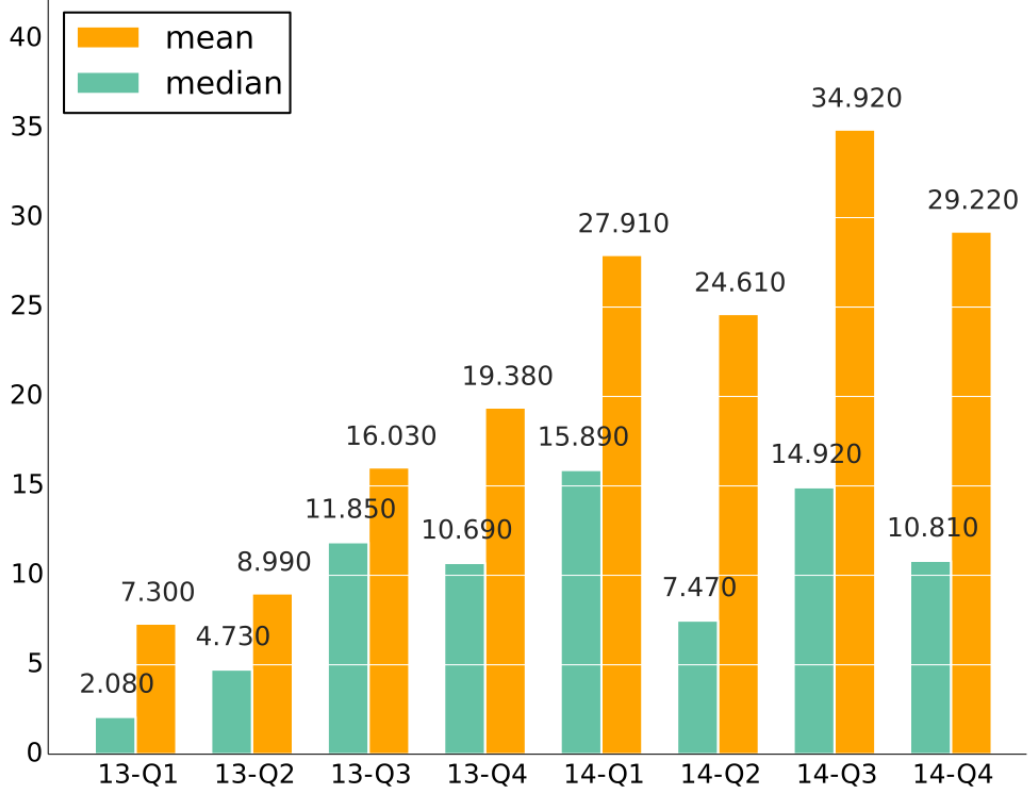
\includegraphics[height=6.5cm]{figs/processes-crs-nova-time-to-merge}
\end{center}

\end{frame}

%%---------------------------------------------------------------

\begin{frame}
\frametitle{Review: time to merge}

\begin{center}
  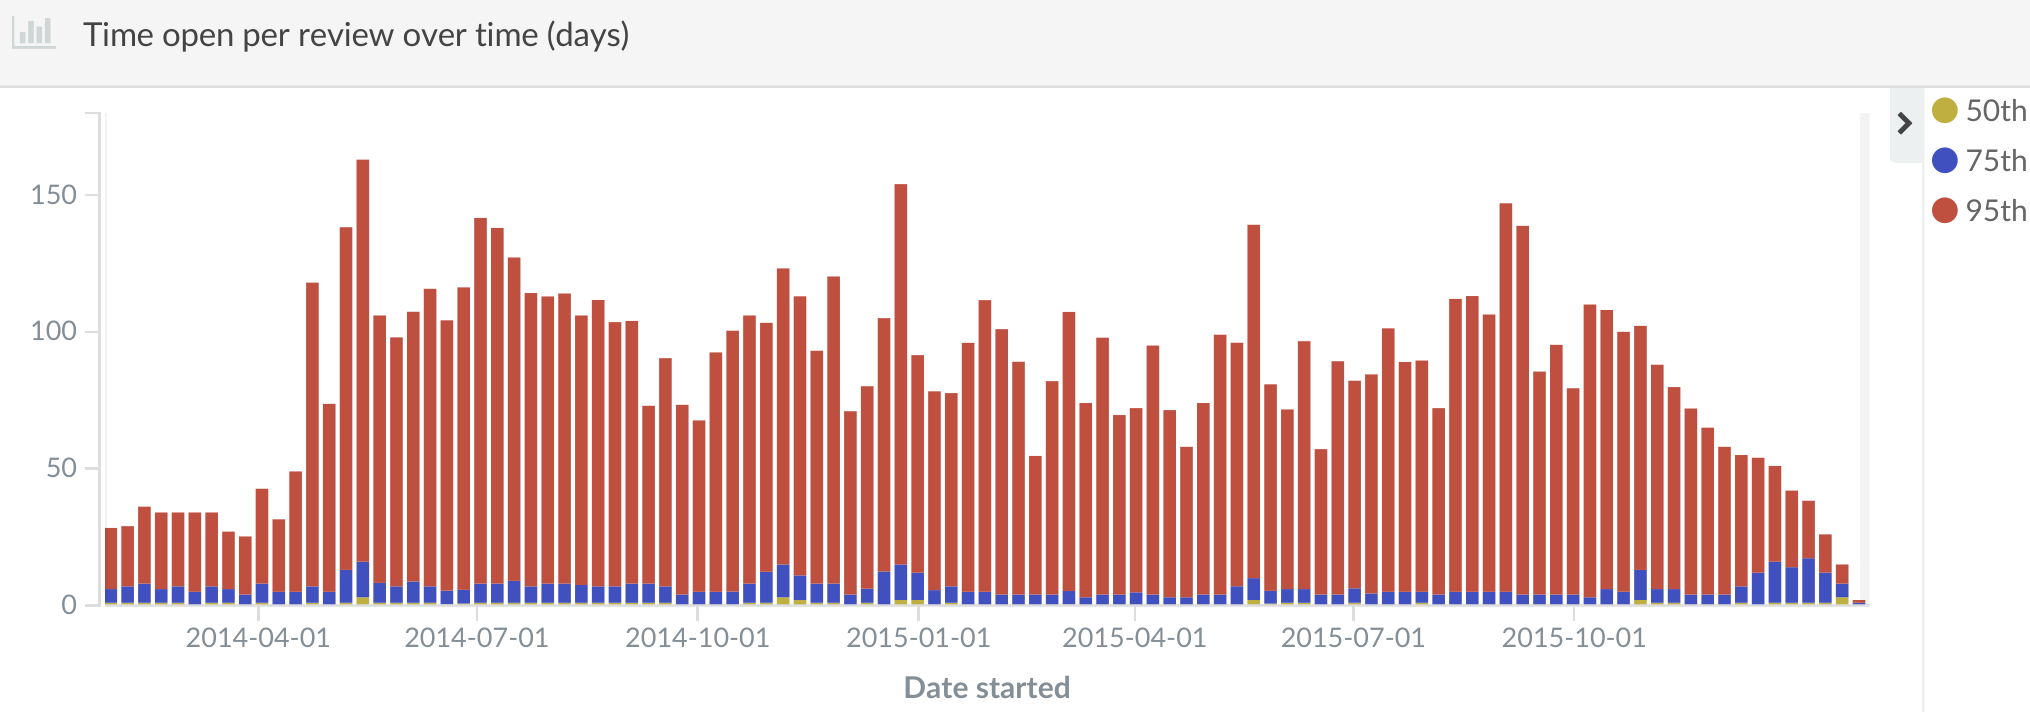
\includegraphics[width=12cm]{figs/timeopen-review}
\end{center}

\end{frame}

%%---------------------------------------------------------------

\begin{frame}
\frametitle{Versions per review}

\begin{center}
  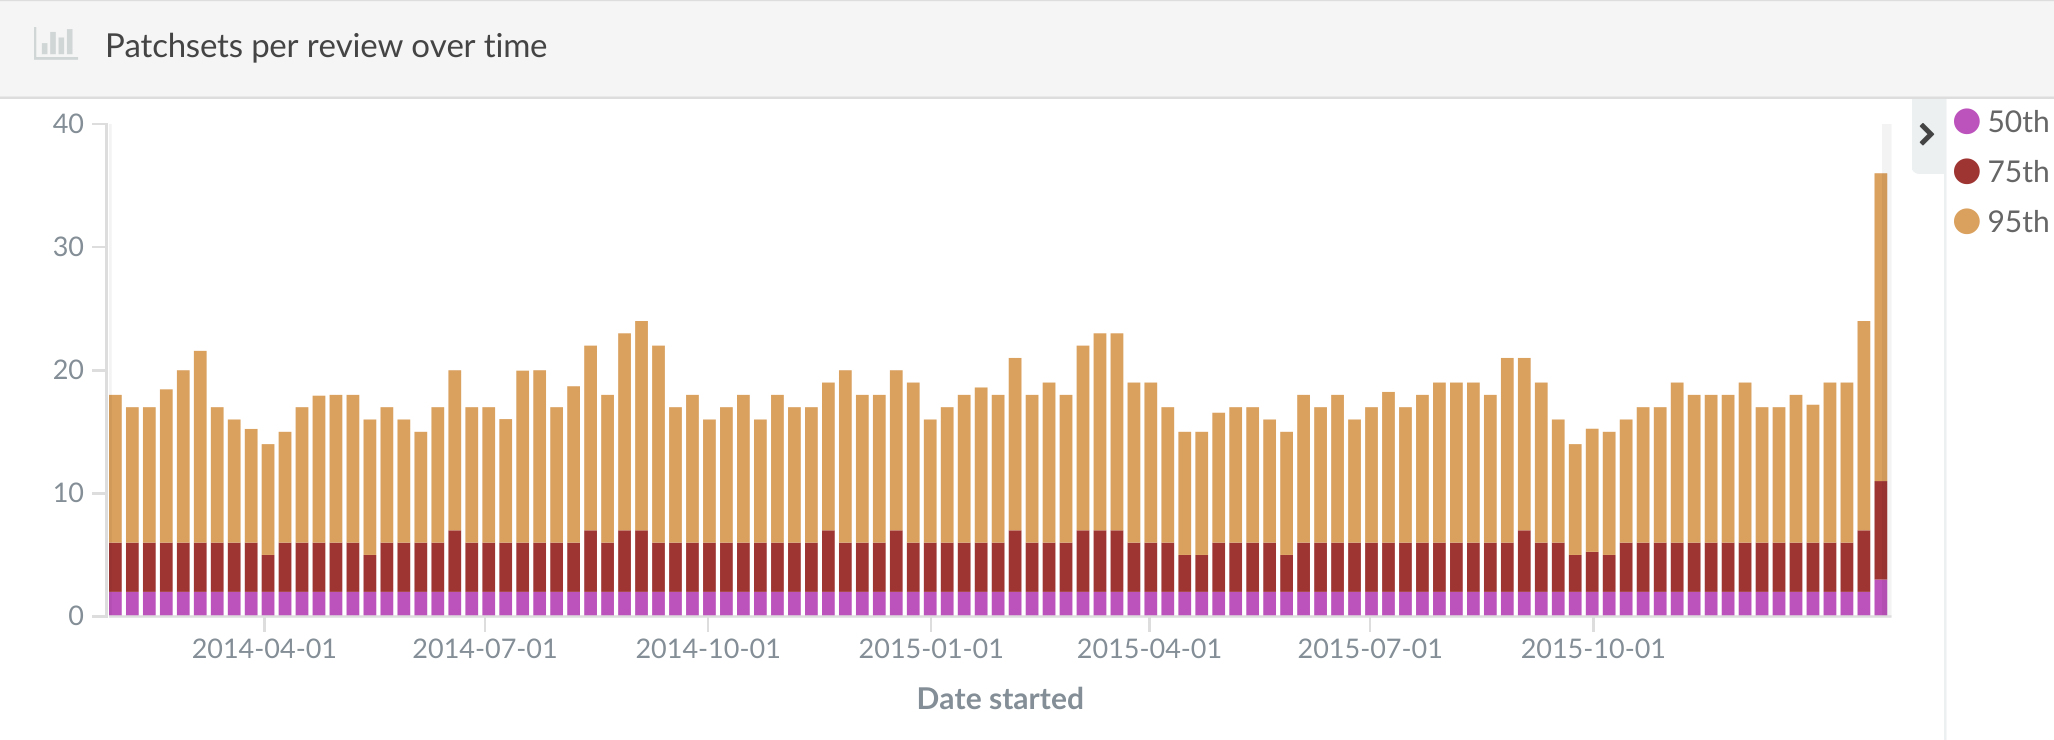
\includegraphics[width=12cm]{figs/patchsets-per-review}
\end{center}

\end{frame}

%%---------------------------------------------------------------

\begin{frame}
\frametitle{The coding process}

\begin{columns}[T]
\begin{column}{.40\textwidth}
{\footnotesize
  From idea to implementation
  
\begin{itemize}
\item Story, design
\item Ticket(s)
\item Code review
\item Automated testing
\item Commit in code base
\end{itemize}
}
\end{column}%
\hfill%
\begin{column}{.58\textwidth}
{\footnotesize
  The OpenStack case

\begin{itemize}
\item Blueprint (if feature), Launchpad
\item Ticket (bug, feature), Launchpad
\item Code review, Gerrit
\item Automated testing, Jenkins
\item Commit in code base, Gerrit, Git
\end{itemize}
}
\end{column}%
\end{columns}

\end{frame}

%%-------------------------------------------------------
%%-------------------------------------------------------
\subsection{Demographics}

%%---------------------------------------------------------------

\begin{frame}

  \begin{itemize}
  \item The repository level.
  \item The class of repository level.
  \item The project level.
  \item The global level.
  \end{itemize}

\begin{center}
  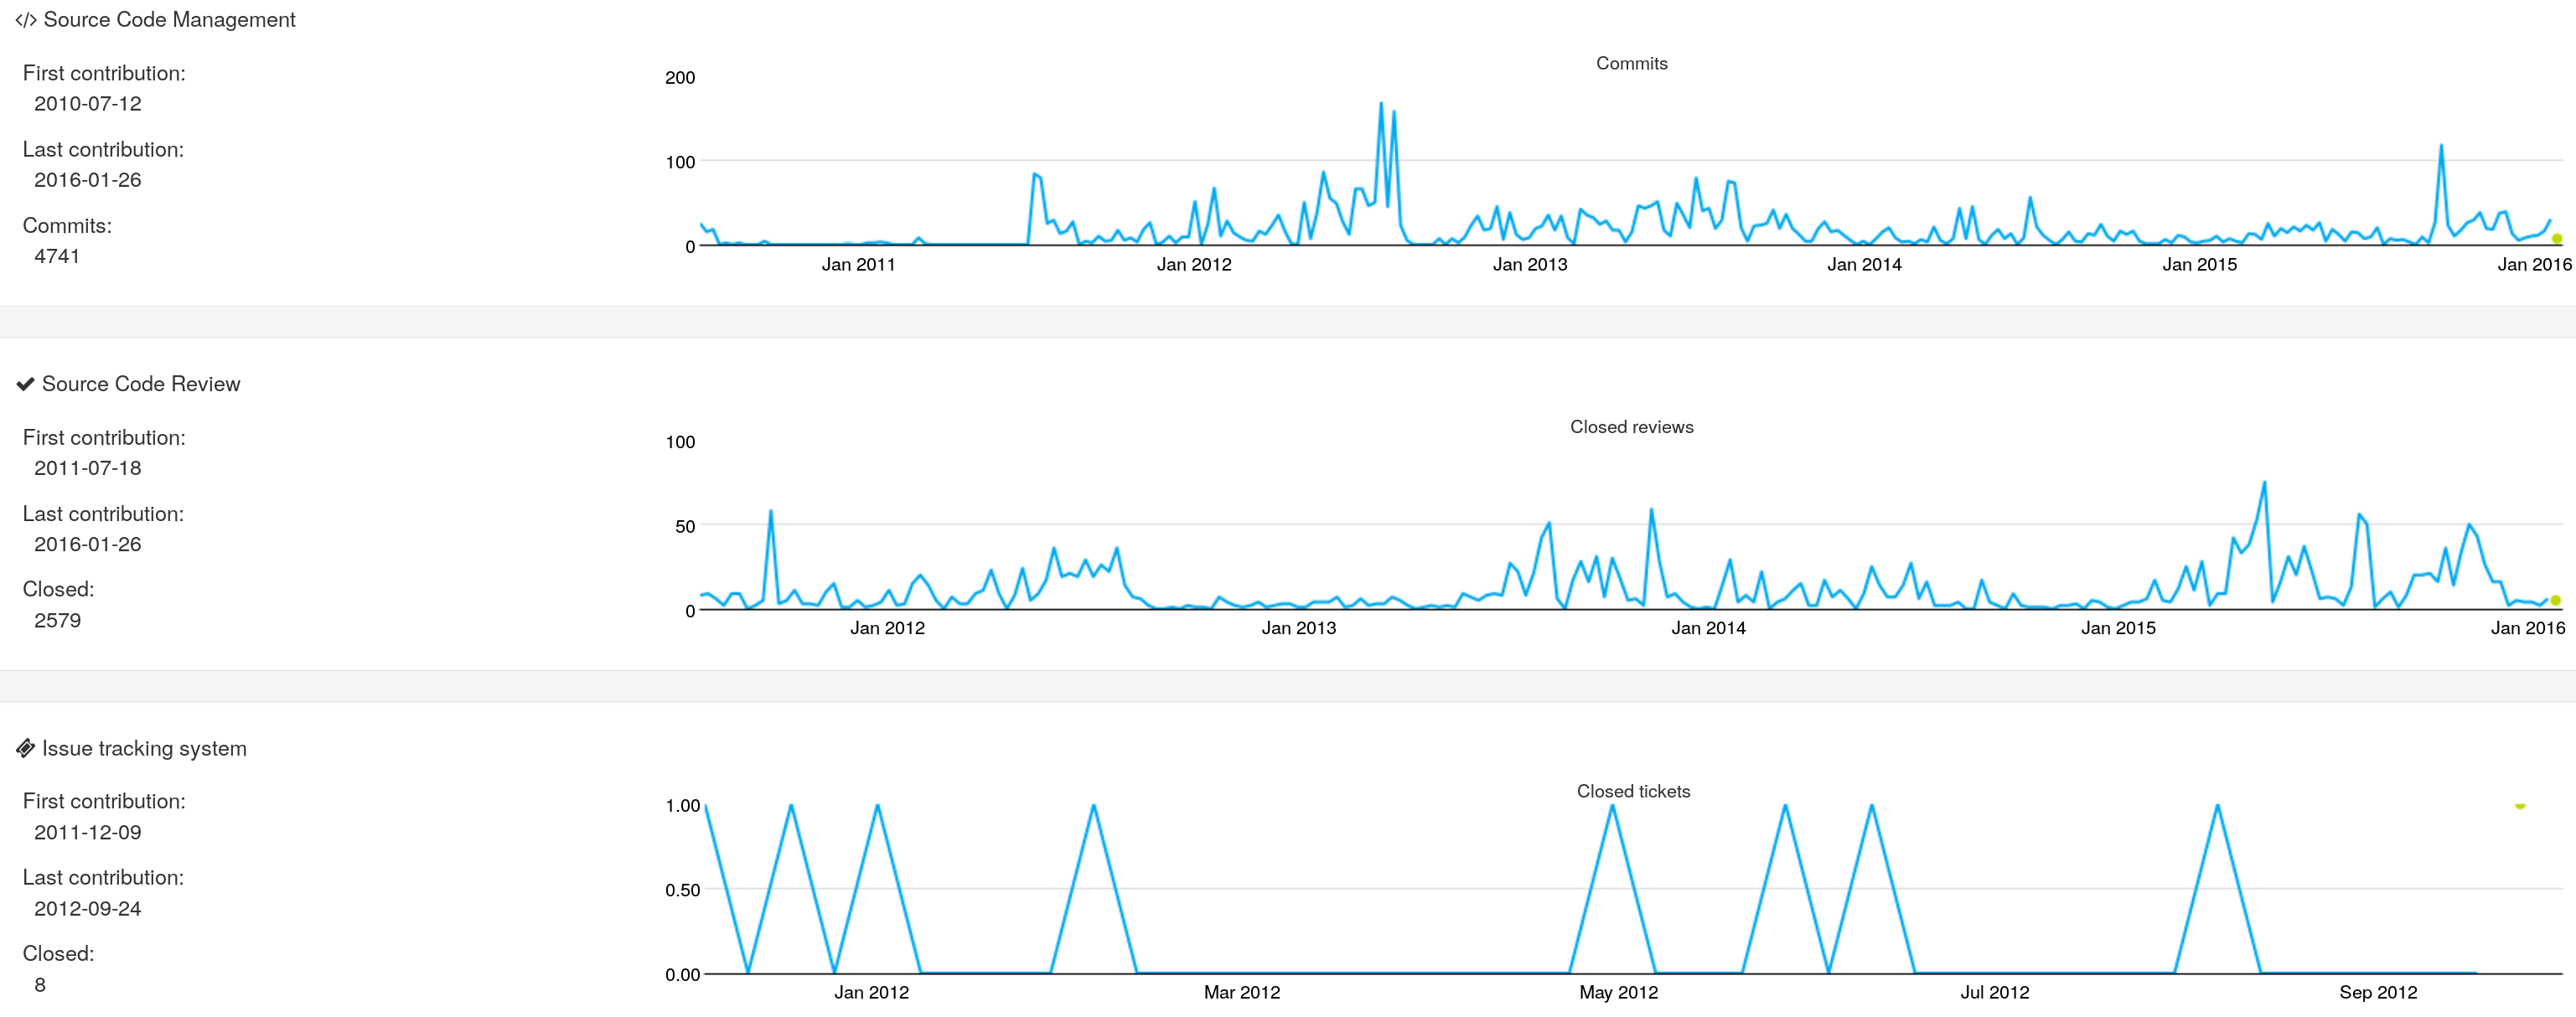
\includegraphics[width=12cm]{figs/person-profile}
\end{center}

\end{frame}

%%---------------------------------------------------------------

\begin{frame}
\frametitle{The aging chart}

\begin{center}
  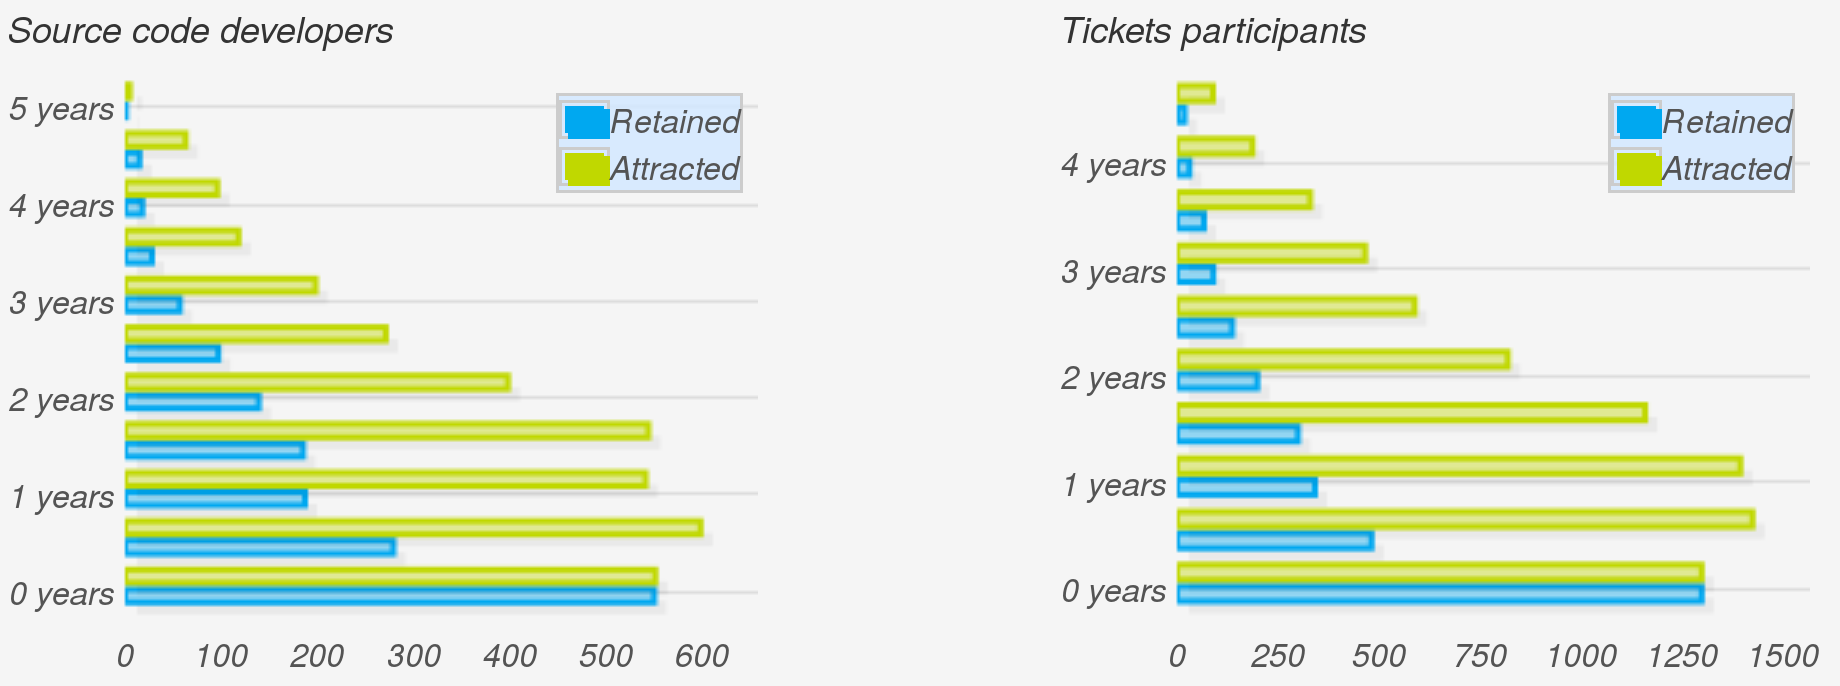
\includegraphics[width=12cm]{figs/aging-openstack}
\end{center}

\end{frame}


%%-------------------------------------------------------
%%-------------------------------------------------------
\subsection{Diversity}

%%---------------------------------------------------------------

\begin{frame}
\frametitle{Time zones}

\begin{center}
  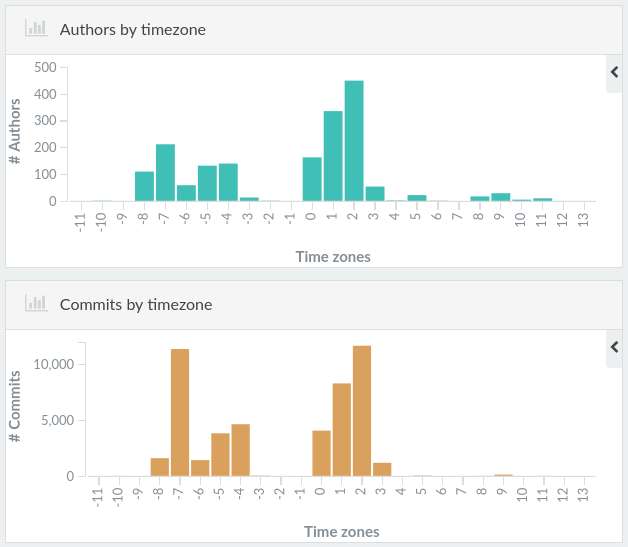
\includegraphics[height=7cm]{figs/elastic-git-tz}
\end{center}

\begin{flushright}
  \url{http://cauldron.io/dashboards/elastic}
\end{flushright}
      
\end{frame}

%%---------------------------------------------------------------

\begin{frame}
\frametitle{GitHub profiles}

\begin{center}
  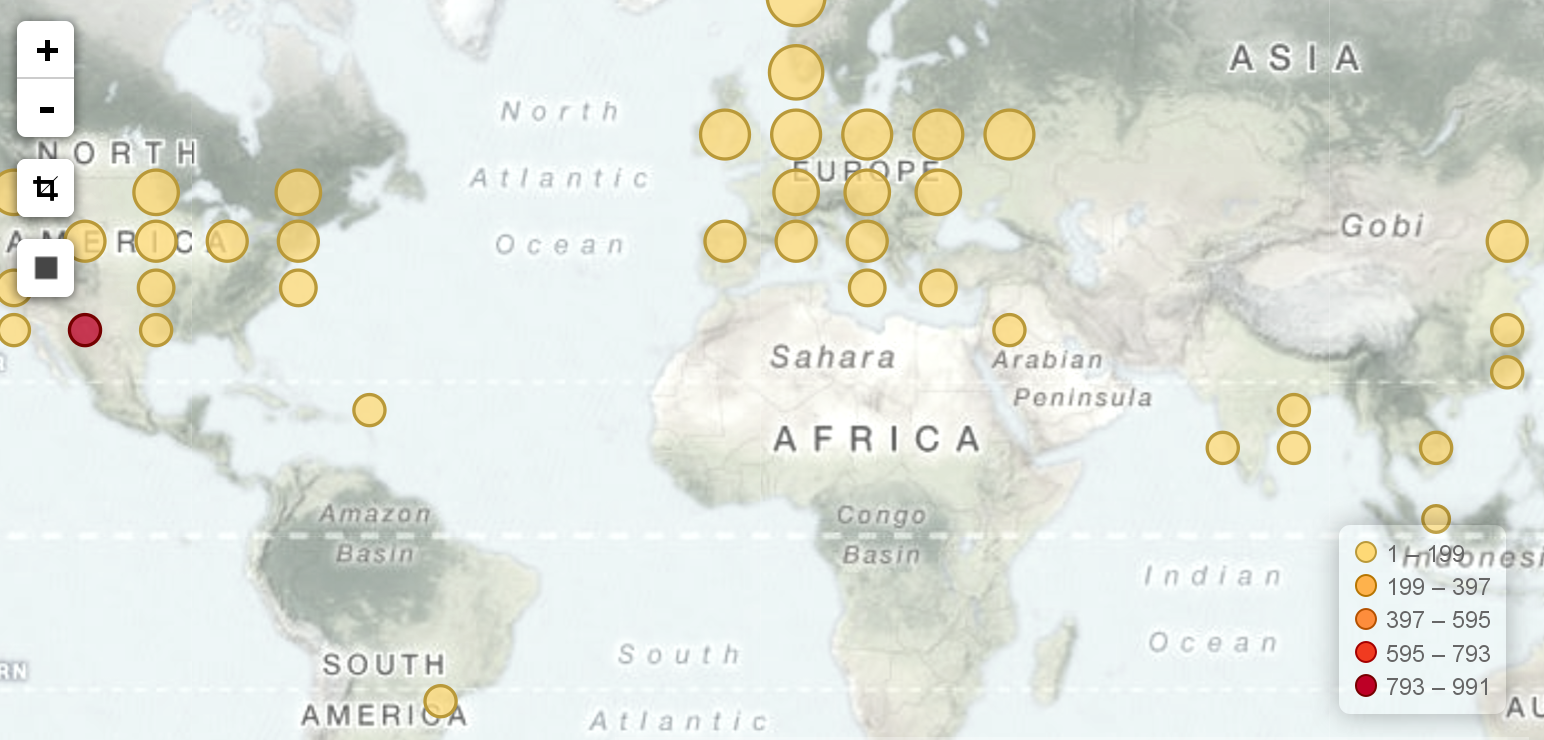
\includegraphics[width=11cm]{figs/map-commits-elasticsearch}
\end{center}

\end{frame}

%%---------------------------------------------------------------

\begin{frame}
\frametitle{Affiliation}

\begin{center}
  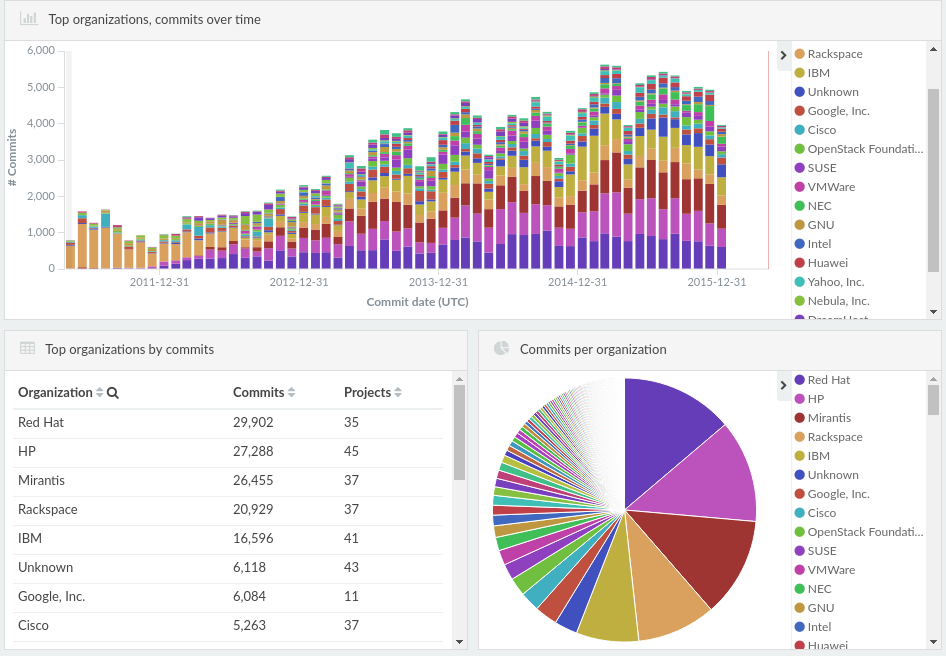
\includegraphics[width=10cm]{figs/organizations-openstack}

\end{center}

\begin{flushright}
  \url{http://s.bitergia.com/db-fosdem16}
\end{flushright}


\end{frame}

%%---------------------------------------------------------------
\begin{frame}
\frametitle{Apache Pony Factor}


% In words of Daniel Gruno:
{\small
\begin{quote}
  Pony Factor (PF) shows the diversity of a project in terms of the division of labor among committers in a project. \\
  \vspace{.2cm}
  Pony Factor is determined as:
  {\bf ``The lowest number of committers whose total contribution constitutes the majority of the codebase''} \\
\end{quote}
}
\footnotesize{
\begin{flushright}
  \href{https://ke4qqq.wordpress.com/2015/02/08/pony-factor-math/}{ke4qqq.wordpress.com/2015/02/08/pony-factor-math/}
\end{flushright}
}
\end{frame}

%%---------------------------------------------------------------
\begin{frame}
\frametitle{Bitergia Elephant Factor}

\begin{center}
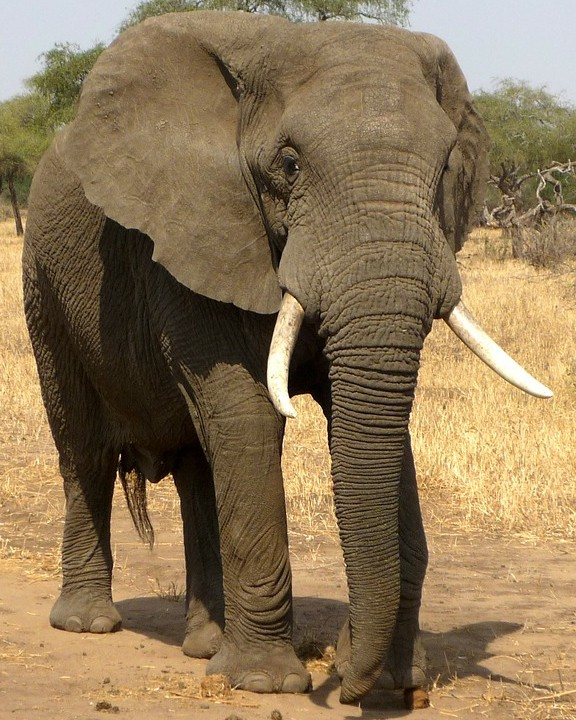
\includegraphics[height=7cm]{figs/elephant}
\end{center}

\end{frame}


%%---------------------------------------------------------------
\begin{frame}
\frametitle{Bitergia Elephant Factor}

{\small
\begin{quote}
The elephant factor shows the diversity of a project in terms of the division of labor among companies (by mean of developers affiliated with them).

  \vspace{.2cm}
  Elephant factor is determined as:\\
  {\bf ``The lowest number of companies whose total contribution (in commits by their employees) constitutes the majority of the commits''} \\
\end{quote}
}
\end{frame}

%%---------------------------------------------------------------
\begin{frame}
\frametitle{Some projects (2016)}

{\footnotesize
\begin{tabular}{|l|l|l|l|l|}
  \hline
              & Pony Factor & Elephant Factor & Commits (excl bots) \\ \hline \hline
OpenNebula    & 4           & 1               & 12K     \\ \hline
Eucalyptus    & 5           & 1               & 25K     \\ \hline
CloudStack    & 14          & 1               & 42K     \\ \hline
OpenStack     & $>$100      & 6               & 126K    \\ \hline
CloudFoundry  & 41          & 1               & 60K     \\ \hline
OpenShift     & 10          & 1               & 15K     \\ \hline
Docker        & 15          & 1               & 18K     \\ \hline
Kubernetes    & 12          & 1               & 7K      \\ \hline
\end{tabular}
}
\end{frame}

%% %%---------------------------------------------------------------
%% \begin{frame}
%% \frametitle{Diversity: Code ``owned''}

%% \begin{columns}[T]
%% \begin{column}{.48\textwidth}
%%   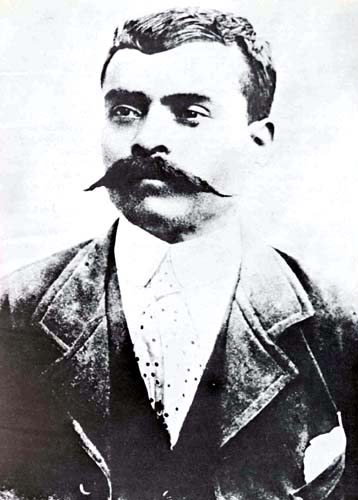
\includegraphics[width=5cm]{figs/emiliano_zapata}
  
%% \end{column}%
%% \hfill%
%% \begin{column}{.50\textwidth}
%%   {\Large \em ``The land belongs \\
%%     to its workers'' \\
%%     \vspace{.4cm}
%%     Emiliano Zapata \\
%%   }
%% \end{column}%
%% \end{columns}

%% \end{frame}

%% %%---------------------------------------------------------------
%% \begin{frame}
%% \frametitle{Diversity: Code ``owned''}

%% {\Large
%%   The code changes over time. The current version is ``owned'' by the people who produced it.\\

%%   \begin{quote}
%%     The code ``belongs'' to those who wrote it.

%%   \vspace{.5cm}
%%   Zapata factor (work in progress): \\
%%   {\bf ``The lowest number of developers for whom the total number of lines of code they ``own'' (were last touched by them) constitutes the majority of the lines of code''} \\
%%   \end{quote}
%% }
%% \end{frame}

%% %%---------------------------------------------------------------
%% \begin{frame}
%% \frametitle{Diversity: Code ``owned''}

%%   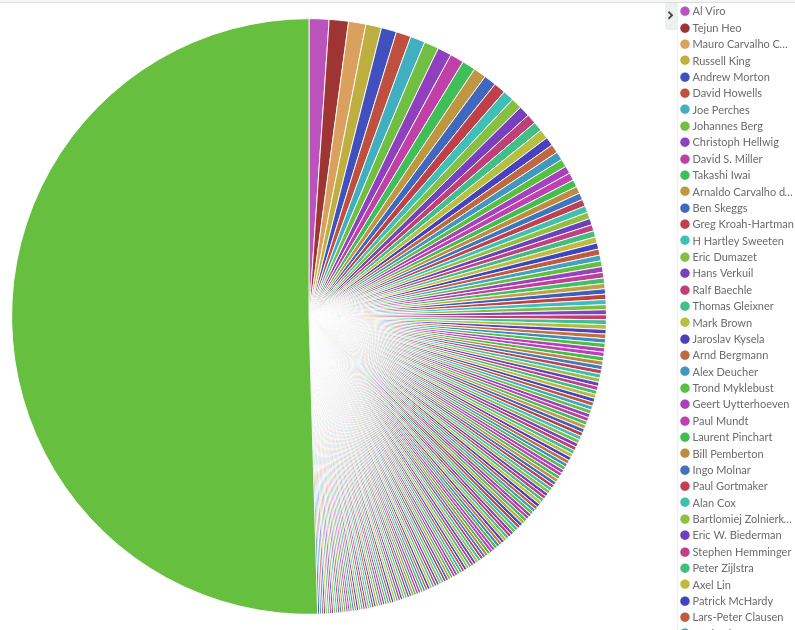
\includegraphics[width=8cm]{figs/linux-authors-pie}

%%   [Linux kernel, July 2016, Zapata factor: 200]
%% \end{frame}

%% %%---------------------------------------------------------------
%% \begin{frame}
%% \frametitle{Diversity: Code ``owned''}

%% {\Large

%%   \begin{quote}
%%     The code ``belongs'' to companies who employ developers changing it.

%%   \vspace{.5cm}
%%   United Fruit factor (work in progress): \\
%%   {\bf ``The lowest number of companies for whom the total number of lines of code they ``own'' (were last touched by their employees) constitutes the majority of the lines of code''} \\
%%   \end{quote}

%% }
%% \end{frame}

%%---------------------------------------------------------------
\begin{frame}
\frametitle{Diversity: Gender gap}

  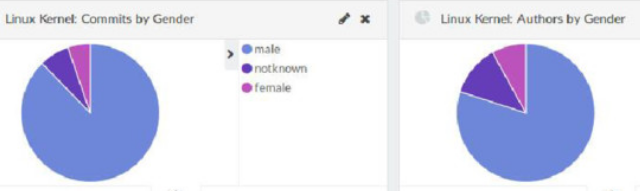
\includegraphics[width=12cm]{figs/linux-gender}
  
    Commits by women: 6.8\% (4 Kcommits) \\
    Women: 9.9\% (330 developers) \\
    Linux kernel, Nov 2015 -- Oct 2016 \\

\end{frame}


%%-------------------------------------------------------
%%-------------------------------------------------------
\section{Final remarks}

%%---------------------------------------------------------------

\begin{frame}
\frametitle{Room for improvement}

  \begin{itemize}
    \item Many other aspects... explore your own
    \item Refine what is important
    \item Explore new ways of making data useful
    \item Tell interesting stories based on data
    \item Visualization is very important
    \item Higher-order metrics
    \item Simplify results, make them meaningful
\end{itemize}

\end{frame}

%%---------------------------------------------------------------

\begin{frame}
\frametitle{Summary}

\begin{center}
  You cannot improve \\
    what you cannot measure \\
\end{center}

\vspace{.2cm}
\begin{flushright}
  Fortunately, you can measure a lot of things...
  \vspace{.5cm}
  
  \url{http://chaoss.github.io/grimoirelab} \\
\end{flushright}

\end{frame}



%%---------------------------------------------------------------

\begin{frame}
\frametitle{Credits (1)}

{\footnotesize
\begin{itemize}
\item ``Man With Two Hats'' \\
  Statue by Henk Visch, located in Otawa, Canada \\
  Picture by Lezumbalaberenjena in Wikimedia Commons \\
  License: Public domain \\
  \url{https://commons.wikimedia.org/wiki/File:Man_With_Two_Hats_Ottawa_Statue_by_lezumbalaberenjena.jpg}
  % two-hats.png

\item ``Crowd at FOSDEM 2008'' \\
  by Jesús Corrius \\
  License: CC Attribution 2.0 \\
  \url{http://www.flickr.com/photos/jcorrius/2302302707/}
  % fosdem-crowd.jpg

%\item {\small ``Emiliano Zapata'' \\
%  License: Public Domain} \\
%  %emiliano_zapata.png

\end{itemize}
}
\end{frame}


\frame{
~
\vspace{1cm}

\begin{flushright}


\includegraphics[width=2.2cm]{figs/by-sa}
 \\

\begin{footnotesize}
\copyright 2016-2019 Jesus M. Gonzalez-Barahona. \\

\vspace{.4cm}

Some rights reserverd. This document is distributed under the terms of the Creative Commons License ``Attribution-ShareAlike 4.0'',
available in \\
{\scriptsize \url{http://creativecommons.org/licenses/by-sa/4.0/}} \\

\vspace{.4cm}

This document (including source) is available from
\url{https://github.com/jgbarah/presentations}

\end{footnotesize}
\end{flushright}

}
%%

%\againframe{firstframe}

\end{document}
